% !TeX root = ./main.tex
% arara: xelatex: { shell : yes }
% arara: bibtex
% arara: xelatex: { shell : yes }
% arara: xelatex: { shell : yes }

% options:
% thesis=B bachelor's thesis
% thesis=M master's thesis
% czech thesis in Czech language
% slovak thesis in Slovak language
% english thesis in English language
% hidelinks remove colour boxes around hyperlinks

\documentclass[thesis=B,czech]{template/FITthesis}[2019/03/06]

\usepackage[utf8]{inputenc} % LaTeX source encoded as UTF-8
\usepackage{dirtree}
\usepackage{minted}
\usepackage{xevlna}
\usepackage[section]{placeins}
\usepackage{hyperref}
\usepackage{enumitem}

\newcommand*{\myAppName}{Totally Not Chernobyl}



% % % % % % % % % % % % % % % % % % % % % % % % % % % % % % 
% NASTAVENI
% % % % % % % % % % % % % % % % % % % % % % % % % % % % % % 

\department{Katedra softwarového inženýrství}
\title{Kooperativní mobilní multiplatformní hra}
\authorGN{Jan} %(křestní) jméno (jména) autora
\authorFN{Bittner} %příjmení autora
\authorWithDegrees{Jan Bittner} %jméno autora včetně akademických titulů
\author{Jan Bittner} %jméno autora bez akademických titulů
\supervisor{Ing. Marek Suchánek}
\acknowledgements{Rád bych na tomto místě poděkoval vedoucímu práce
Ing. Markovi Suchánkovi za cenné rady a přátelský přístup.
Také bych rád poděkoval své rodině za podporu během studia.
}
\abstractCS{Práce se zabývá návrhem a implementací kooperativní mobilní multiplatformní hry
pro mobilní operační systémy Android a iOS
s využitím multiplatformního frameworku Flutter.
Důraz je kladen také na výběr a popis možností
frameworku, state managementu, databáze, architektury a testování.
}
\abstractEN{The thesis describes design and implementation of cooperative mobile
multi-platform game for Android and iOS mobile operating systems
using the multi-platform Flutter framework.
Emphasis is also placed on the selection and description of
framework, state management, database, architecture and testing options.
}
\placeForDeclarationOfAuthenticity{V~Praze}
\declarationOfAuthenticityOption{4} %volba Prohlášení
\keywordsCS{mobilní multiplatformní hra, kooperace,
Flutter, Android, iOS, Cloud Firestore
}
\keywordsEN{mobile multi-platform game, cooperation,
Flutter, Android, iOS, Cloud Firestore
}
\website{https://github.com/tenhobi/bachelors-thesis} %volitelná URL práce, objeví se v tiráži

% % % % % % % % % % % % % % % % % % % % % % % % % % % % % % 
% OBSAH
% % % % % % % % % % % % % % % % % % % % % % % % % % % % % %  

\begin{document}

%https://github.com/tenhobi/bachelors-thesis/issues/11
\begin{introduction}
Poslední desetiletí jsou mobilní telefony nedílnou součástí všedního dne.
Telefony používáme pro práci, komunikaci na sociálních sítích i zábavu.
Obchody s aplikacemi obsahují obrovské množství aplikací a her,
které si může každý stáhnout během několika chvil.
Velkou část aplikací lze stáhnout i bezplatně,
případně lze bezplatně stáhnout alespoň určitou část hry.

Podle statistik a trendů z herního odvětví \cite{wepc_video_game_statistics}
lze vidět,
že na světě je přes 2,5 miliardy hráčů.
77 \% uživatelů mobilních zařízeních jsou hráči,
přičemž v roce 2013 to bylo pouhých 52,3 \% uživatelů.
76 \% lidí preferuje hrát hry na mobilních zařízeních,
oproti 62\% lidí, kteří preferují hraní na PC.
Průměrný věk hráčů je 33 let, průměrný věk hráček je 37 let.
92 \% her dostupných na obchodě Google Play bylo zdarma ke stažení.

Z těchto trendů vyplývá motivace pro vývoj právě mobilní hry,
která je zaměřena především na mladší část publika,
je dostupná zdarma a je snadná na pochopení i hraní,
což umožní poskytnout hru více potencionálním hráčům.

Tato práce se zaměřuje na analýzu, návrh, implementaci a testování
multiplatformní mobilní herní aplikace s prvky kooperace.
Aplikace je určena pro převážně mladší hráče
a je navžena dostatečně jednoduše,
aby byla nenáročná a tím více atraktivní.

Práce je rozdělena do 7 kapitol.
V první kapitole je rozebrán výběr čtyř konkurenčních aplikací,
včetně zhodnocení kladů a záporů jednotlivých her.
Tato rešerše pomáhá k inspiraci pro vytvoření lepšího zážitku pro navrhovanou
hru.
V druhé kapitole jsou popsány možnosti technologií,
které lze využít pro praktickou část práce.
Jednoltivé typy technologií jsou na závěr každé podkapitoly zhodnoceny
a jsou vysvětleny procesy, které vedly k výběru právě dané technologie.
Ve třetí kapitole je provedena analýza hry, požadavků a případů užití.
Čtvrtá kapitola je zaměřena na návrh uživatelského rozhraní a architektiry.
Obě části mají detailněji rozebrány zajímavé vybrané části při návrhu.
Pátá kapitola se zabývá popisem použitých nástrojů
a jednotlivých přínosů, který daný nástroj přináší.
Jsou popsány použité knihovny, které kvalitně řeší dílčí části.
A v neposlední řadě je představeno několik vybraných zajímavých
implementačních částí.
Šestá kapitola je zaměřena na testování.
V kapitola jsou popsány použité typů testů,
uživatelské testování a především jsou představeny vybrané ukázky testů
implementace.
V poslední, sedmé, kapitole se čtenář dozvídá o způsobech nasazení a
možnostech distribuce aplikace pro mobilní operační systémy Android a iOS.

V závěru práce je pak zhodnocení výsledků práce a možnosti rozšíření.
Důležitou součástí jsou také splněné cíle.
\end{introduction}

\chapter{Cíle práce}

Cílem práce je analýza, návrh a implementace funkční
kooperativní multiplatformní mobilní herní aplikace,
ve které se hráči připojí do místnosti a společně se snaží splnit mise hry.

Nejprve jsou v rámci teoretické části práce zhodnoceny klady a zápory
konkurenčních aplikací,
aby bylo zjištěno,
kde je vhodné se motivovat, a čemu se naopak vyvarovat.
Dalším úkolem je získání přehledu o moderních technologiích
a provedení rešerše možností, jednotlivě je prozkoumat a popsat
a na závěr každé technologie zhodnotit nejvhodnější výběr.
Neméně důležitý je také úkol samotného navrhnutí principů a logiky hry,
jejích funkcí, požadavků na aplikaci a případů užití.

Praktická část má za úkol vhodně navrhnout architekturu aplikace
a uživatelské rozhraní a následně provést implementaci řešení tak,
aby byla aplikace plynulá, udržitelná a snadno rozšiřitelná.
Dalším úkolem je také aplikaci řádně otestovat automatizovanými testy 
a provést uživatelské testování.

V neposlední řadě je úkolem také vytvoření uživatelské a vývojářské
dokumentace.

% !TeX root = ../main.tex
\chapter{Konkurenční aplikace}

Po prozkoumání podobného žánru her
– kooperace, komunikace a rychlost reakcí –
dostupných v obchodě Google Play,
byly vybrány konkurenční herní aplikace.
Tyto hry byly vybrány zejména podle popularity a počtu stažení v obchodě
a podle subjektivně vnímaného potenciálu,
který má daná hra k inspiraci pro tvorbu herní aplikace.

V následujících sekcích budou popsány vybrané 4 konkurenční aplikace,
včetně shrnutí kladů a záporů.

\section{DUAL!}

První vybranou hrou je \emph{DUAL!}.
Tato hra využívá zejména prvky kooperace a rychlosti reakcí
a je velmi akčně laděná.
Jak říká první věta stránky hry \cite{seabaa_dual} v obchodě Google Play:
\uv{Mezi lidmi, napříč obrazovkami.}

Hra se rozprostírá přes 2 obrazovky zařízení a herní postava se ovládá natáčením
daného displeje.
Pokud například postava vystřelí na jedné obrazovce,
střela za chvíli doletí i na obrazovku druhou.
Vyvolání příslušných akcí se ovládá určitými kombinacemi dotyků na displej.

UI je velmi jednoduché, avšak přívětivé svými barvami a srozumitelností.
Všechny prvky jsou pochopitelné.

\myFigure{Alpha}{fig:dual}{assets/competitive-apps/dual.jpg}
\FloatBarrier

\subsection{Klady}

TODO text

\subsection{Zápory}

TODO text

\section{Sea Battle 2}

Hra \emph{Sea Battle 2} sice není postavena na kooperaci a komunikaci mezi
hráči,
ale představuje hezkou reprezentaci klasické deskové hry v moderním pojetí
\cite{henrysmithinc_spaceteam}.

Hráči z celého světa mezi sebou na svých zařízeních vedou souboje a vítězstvími
postupně postupují v námořních hodnostech.
Oproti klasické verzi hra disponuje i pokročilým módem,
který obsahuje nejrůznější letadla a pokročilé děla,
které obohatí hru o nové strategie.

UI je lazeno do podoby čtverečkovaného papíru s ručně kreslenými prvky,
což ale nepůsobí moc přívětivě a tvoří několik problémů,
mezi nimiž je například nemožnost přiblížení,
což velmi komplikuje některé úkony.

\myFigure{Alpha}{fig:sea-battle}{assets/competitive-apps/sea-battle.jpg}
\FloatBarrier

\subsection{Klady}

TODO text

\subsection{Zápory}

TODO text

\section{Keep Talking and Nobody Explodes}

Ve hře \emph{Keep Talking and Nobody Explodes} závisí všechno na správné
kooperaci a komunikaci.
Tato velmi oceňovaná hra existuje ve verzi pro desktop, konzole,
virtuální realitu i mobily \cite{steelcrategamesinc_keep}.

Cílem hry je zneškodnění bomby.
Jeden hráč vidí bombu, která je koncipována jako kufřík s několika moduly
a časomírou, která se nebezpečně rychle odpočítává.
Další hráč, případně skupina, mají k dispozici manuál s instrukcemi.
Manuál mohou prohlížet jak v elektronické, tak i ve vytištěné podobě.
Manuál je totiž pro všechny hry shodný.

Veškerá komunikace probíhá pouze slovně.
Hráč s bombou tak nahlásí hráči s manuálem například to,
že vidí červené tlačítko s textem \uv{defuse}.
Druhý hráč pak v manuálu vyhledá daný modul tlačítka, řídí se instrukcemi a
podstatné informace předá prvnímu hráči.

\myFigure{Alpha}{fig:keep-talking}{assets/competitive-apps/keep-talking.jpg}
\FloatBarrier

\subsection*{Klady}

\begin{itemize}
    \item UI je laděné jako pohled na stůl, na kterém je bomba a časomíra,
což dodává atmostféru a vtáhne hráče do děje.
    \item Světla v místnosti blikají, případně se vypínají.
To přidává efekt zejména v situácích,
kdy zbývá už jen pár sekund a bomba není vidět.
    \item Přestože je grafika jednodušší, samotná bomba je velmi přehledná.
\end{itemize}

\subsection*{Zápory}

\begin{itemize}
    \item U složitějších modulů je manuál občas hůře pochopitelný.
\end{itemize}

\section{Spaceteam}

Poslední hra, \emph{Spaceteam}, stojí na rychlosti reakcí a velmi rychlé
komunikaci, což shrnuje první věta na stránce hry \cite{henrysmithinc_spaceteam}
v obchodě Google Play: \uv{Mačkáš rád tlačítka a řveš na své kamarády?}

Herní plocha je plná náhodných tlačítek, přepínačů, posouvátek a dalších věcí,
se kterými musí hráči pracovat podle přicházejících příkazů.

Zapeklitost komunikace spočívá v tom,
že příkazy se netýkají pouze prvků na nadaném zařízení,
ale i prvků ze zařízení ostatních lidí.
Některé příkazy také cílí na všechny hráče.
Příkladem takévého příkazu je například zatřesení všemi zařízeními najednou.

\myFigure{Screenshot hry Spaceteam}{fig:spaceteam}{assets/competitive-apps/spaceteam.jpg}
\FloatBarrier

\subsection*{Klady}

\begin{itemize}
    \item UI úvodní obrazovky a přihlašování do hry vypadá velmi efektně.
    \item Tlačítka i příkazy obsahují řadu technologických pojmů,
což dodává hře na správné atmosféře.
\end{itemize}

\subsection*{Zápory}

\begin{itemize}
    \item Herní obrazovka má poněkud zastaralé, až nevkusné, prvky.
    \item Hra probíhá až příliš rychle.
Nutno přiznat, že tento fakt není nutně nevýhoda,
avšak ubírá to na prvku kvalitnější komunikace.
    \item Hra nemá možnost přihlášení,
a tedy shromažďování a uchovávání statistik.
\end{itemize}

\chapter{Rešerše technologií}

Tato kapitola je věnována rešerší jednotlivých skupin technologií,
které budou použity v rámci praktické části.
V každé podkapitole jsou shrnuty možnosti, klady a zápory
jednotlivých technologií a na závěr je provedeno zhodnocení.

\section{Multiplatformní framework}

Vývoj mobilních aplikací je dle~\cite{wepc_video_game_statistics} na vzestupu.
To přináší nároky na vydavatele a vývojáře k rychlejší tvorbě mobilních
aplikací a her.
Aplikace pro mobilní zařízení se běžně vytvářejí pomocí programovacích jazyků,
které jsou úzce spjaty
s mobilními zařízeními~\cite{dashmagazine_mobile_frameworks}.
Příkladem takového programovacího jazyka je jazyk Java,
který se používá pro vývoj nativních aplikací
v platformě Android~\cite{dashmagazine_mobile_frameworks}.
Tyto jazyky mají úzkou podporu pro vývoj na daných zařízeních,
včetně přístupu k hardwarovému rozhraní (kamera, senzory, \dots{}),
jak uvádí zdroj~\cite{dashmagazine_mobile_frameworks}. 

\begin{figure}[ht!]
    \centering
    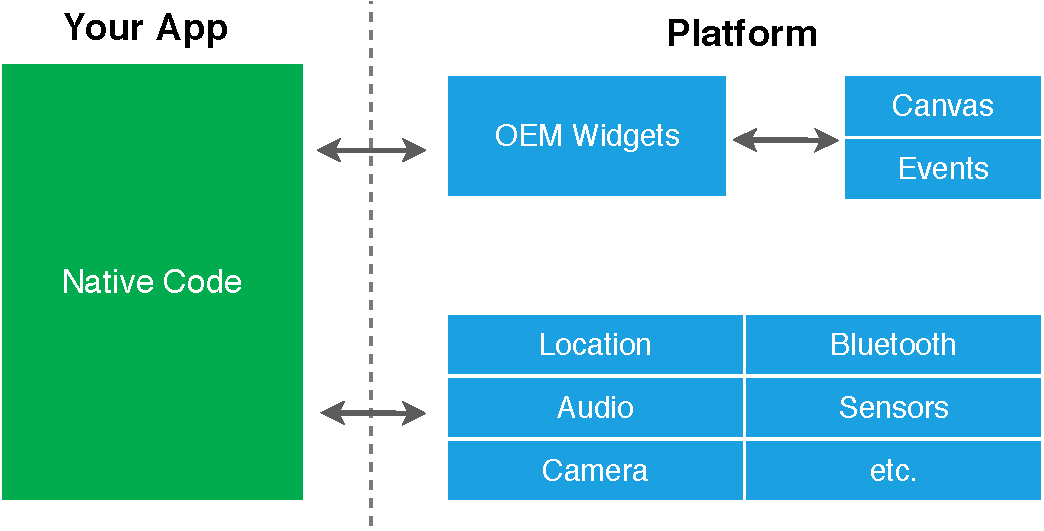
\includegraphics[width=\linewidth]{assets/technology-research/framework/platform_sdk.pdf}
    \caption{Schéma frameworku specifického pro platformu~\cite{hackernoon_flutter}}
    \label{fig:framework_platform}
\end{figure}

Snahu urychlit vývoj mobilních aplikací řeší také mobilní frameworky.
Tyto frameworky jsou tvořeny většinou stejnou společností,
která také vytváří danou platformu,
a jsou publikovány jako \emph{Software Development Kit} (dále jen SDK).
Pro platformu Android je vyvíjeno Android SDK,
spolu s podpůrnými programy jako integrované vývojové prostředí
(dále jen IDE) a emulátory.
Tyto frameworky jsou díky jejich úzkému propojení a plné kompatabilitě
považovány za rychlé,
avšak mnohdy vyžadují speciální znalosti pro konkrétní platformu.
Právě cílení výhradně na danou platformu je největší nevýhoda těchto typů
frameworků.
Na obrázku~\ref{fig:framework_platform} lze vidět architekturu těchto
frameworků.~\cite{dashmagazine_mobile_frameworks}

Další snahou pro ještě rychlejší a snadnější vývoj aplikací jsou frameworky
s podporou multiplatformnosti,
a tedy frameworky cílící na více platforem~\cite{hackernoon_flutter}.
To může být pouze cílení na mobilní platformy,
ale dokonce také i cílení na web, osobní počítače a další.
Tyto frameworky podporují populární jazyky,
umožňují sdílet kód mezi jednotlivými platformami
a v závislosti na architektuře se blíží rychlostí výsledných aplikací
k aplikacím psaných nativními jazyky~\cite{hackernoon_flutter}.
Pomocí těchto technologií lze tedy vyvíjet aplikace pohodlně, rychle
a benefitem \uv{zadarmo} je podpora multiplatformnosti vyvíjené
aplikace~\cite{dashmagazine_mobile_frameworks}.

\begin{figure}[ht!]
    \centering
    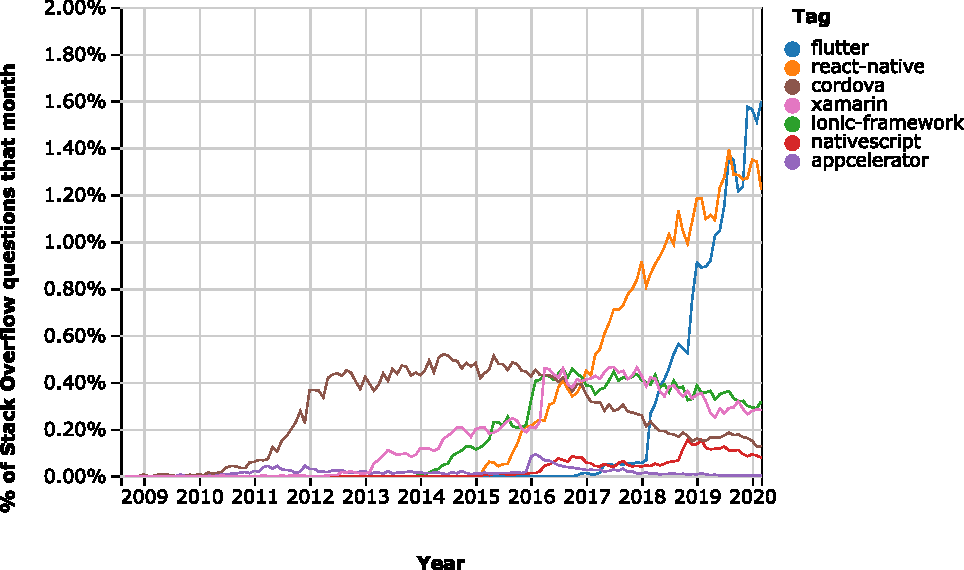
\includegraphics[width=\linewidth]{assets/technology-research/framework/popularity.pdf}
    \caption{Vývoj trendu multiplatformních
    frameworků~\cite{framework_popularity}}
    \label{fig:framework_popularity}
\end{figure}

V následujících sekcích je vybráno a popsáno několik multiplatformních
frameworků.
Tyto frameworky byly vybrány na základě trendů~\cite{framework_popularity}
na síti Stack Overflow.
Na obrázku~\ref{fig:framework_popularity} lze vidět reprezentace těchto trendů,
ve kterých lze vyčíst,
jak se trend pro daný jazyk vyvíjí v čase.
Nejvíce populární na této síti je tedy framework Flutter,
který překonal popularitu frameworku React Native,
avšak oba frameworky si udržují dlouhodobý růst.
Ostatní frameworky si trend udržují,
nebo jim dokonce klesá.

\subsection{Ionic}

\begin{figure}[ht!]
    \centering
    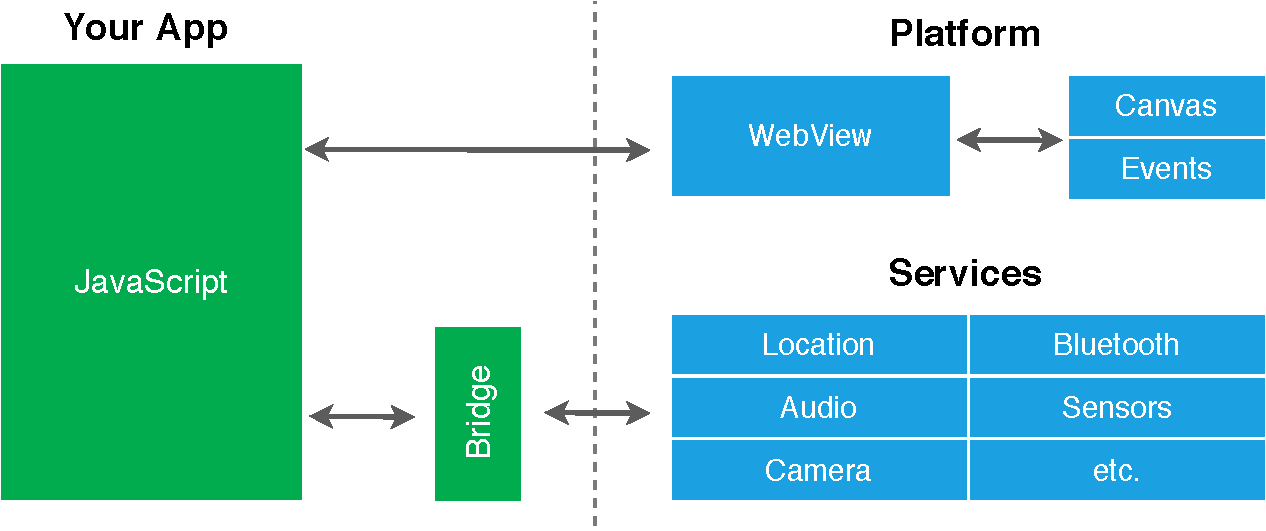
\includegraphics[width=\linewidth]{assets/technology-research/framework/webview.pdf}
    \caption{Schéma architektury s WebView~\cite{hackernoon_flutter}}
    \label{fig:framework_webview}
\end{figure}

První multiplatformní frameworky začaly pro multiplatformnost využívat
WebView~\cite{hackernoon_flutter}.
Tyto frameworky aplikaci vykreslují pomocí webových technologií
a komunikaci s hardwarovým rozhraním řeší pomocí speciálního komunikačního
mostu~\cite{hackernoon_flutter}.
Taková architektura je vidět na obrázku~\ref{fig:framework_webview}.
Z tohoto obrázku jde vidět,
jak moc je zdrojový kód oddělený od dané platformy.

Jedním z představitelů těchto frameworků je i framework Ionic,
který je stále značně využívaný i v dnešní době,
dle trendů z obrázku~\ref{fig:framework_popularity}.
Framework Ionic využívá jazyky jako HTML, CSS a JavaScript.
V tomto frameworku je možné vytvořit aplikaci pro mobilní platformy
Android a iOS.
Významnou výhodou je,
že díky využití mobilních technologií,
které se používají naprosto shodně jako při vývoji webových aplikací,
se nemusí vývojáři učit nové technologie a přístupy k vývoji,
čímž se také celý proces zrychlí.
Důsledkem používání webových technologií jsou ale i jejich nevýhody,
zejména nižší výkon.~\cite{dashmagazine_mobile_frameworks}

S frameworkem Ionic lze využít také frontend knihovny a frameworky.
Příkladem jsou knihovny a frameworky React, Angular či Vue.
Součástí je také knihovna komponent UI,
které se automaticky přizpůsobí dané platformě.
Součástí jsou také podpůrné konzolové nástroje pro vytváření, produkování a
testování aplikací.~\cite{ionic}

\subsection{React Native}

Další přístup k vývoji multiplatformních aplikací představuje framework
React Native.
Tento framework využívá pomocí komunikačního mostu nativní komponenty platformy
díky vzorům z reaktivního programování zjednodušuje celkový
vývoj~\cite{hackernoon_flutter}.
Framework je založen na populární webové
knihovně ReactJs~\cite{dashmagazine_mobile_frameworks}.
Jelikož framework nepoužívá nativní komponenty platformy,
a tedy ani WebView,
jsou aplikace produkované tímto frameworkem
rychlejší~\cite{dashmagazine_mobile_frameworks}.
Pro popis UI je používán vlastní jazyk založený na XML,
nazývaný JSX~\cite{dashmagazine_mobile_frameworks}.

\begin{figure}[ht!]
    \centering
    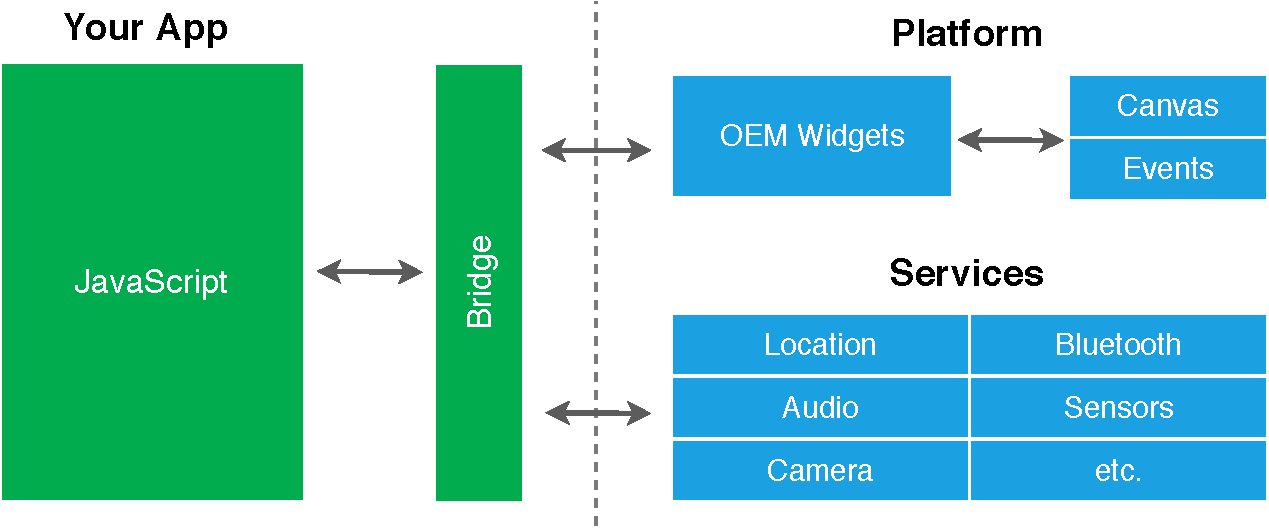
\includegraphics[width=\linewidth]{assets/technology-research/framework/react_native.pdf}
    \caption{Schéma architektury frameworku React Native~\cite{hackernoon_flutter}}
    \label{fig:framework_react_native}
\end{figure}

Framework React Native obsahuje \emph{hot reloading},
což je vlastnost,
která umožní vidět všechny změny ihned po jejich změně,
bez zbytečně zdlouhavého procesu sestavování celé aplikace.
K dispozici je také velká škála komponent,
včetně velkého množství komponent od vývojářů třetí strany, 
které mohou vývojáři volně používat.~\cite{dashmagazine_mobile_frameworks}

Framework byl vytvořen v roce 2015
společností Facebook,
která jej od té doby spravuje~\cite{hackernoon_flutter}.
Za zmíňku stojí populární aplikace,
které framework využívají,
mezi nimi jsou například mobilní aplikace Facebook, Instagram, Skype, Discord
a mnoho dalších~\cite{react_native}.

Na obrázku~\ref{fig:framework_react_native} lze vidět schéma architektury
frameworku React Native.
Jak lze z obrázku vyčíst,
tato architektura,
oproti architektuře s WebView,
komunikuje s platformou kompletně přes komunikační most pomocí jazyku
JavaScript.

\subsection{Flutter}

Posledním frameworkem je Flutter,
který je vyvíjený společností Google.
Tento framework je nejmladším z představených frameworků,
avšak dle trendů z obrázku~\ref{fig:framework_popularity},
kde je vidět razantní nárůst,
se jim minimálně snadno vyrovná.
Framework Flutter přistupuje k multiplatformnosti jinak,
než ostatní mobilní frameworky.
Nejenže tento framework nevyužívá programovací jazyk JavaScript,
což samo o sobě přináší řadu výhod,
ale také přesouvá starost s vykreslováním z platformy na framework
\cite{hackernoon_flutter},
jak lze vidět na obrázku s reprezentací
architektury~\ref{fig:framework_flutter},
a také se plně kompiluje do nativního
kódu~\cite{dashmagazine_mobile_frameworks}.
Podporované nejsou pouze mobilní platformy Android a iOS,
ale také platformy web a desktop~\cite{flutter}.
Platforma web je momentálně dostupná ve verzi beta,
platforma desktop je dostupná ve verzi alfa~\cite{flutter_web, flutter_desktop}.

\begin{figure}[ht!]
    \centering
    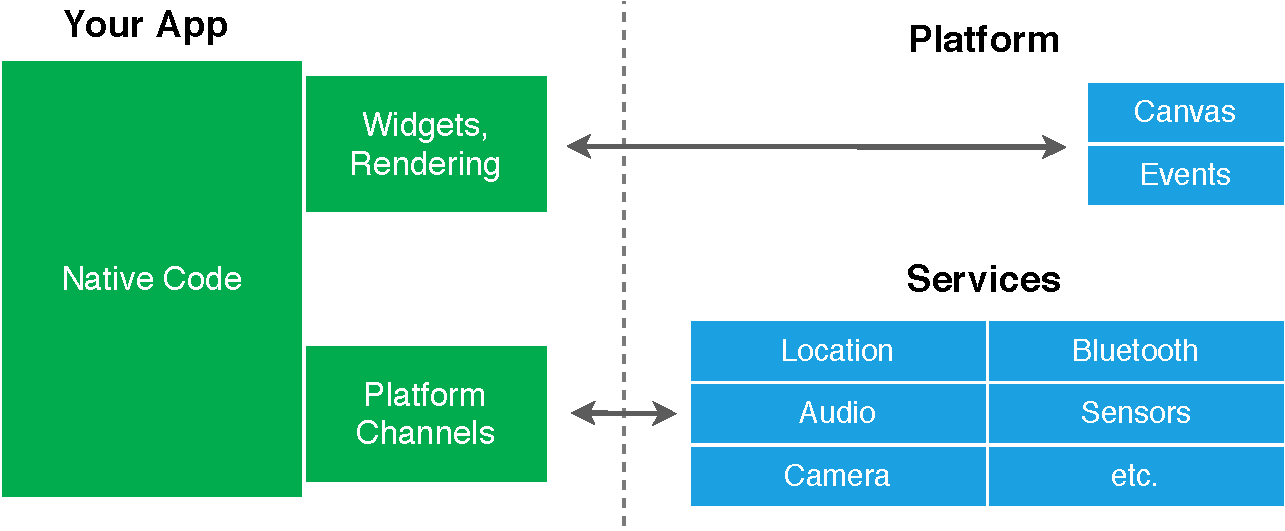
\includegraphics[width=\linewidth]{assets/technology-research/framework/flutter.pdf}
    \caption{Schéma architektury frameworku Flutter~\cite{hackernoon_flutter}}
    \label{fig:framework_flutter}
\end{figure}

Framework Flutter využívá programovací jazyk Dart,
který umožňuje jak kompilaci \emph{ahead of time} (dále jen AOT),
tak i kompilaci \emph{just in time} (dále jen JIT)~\cite{hackernoon_flutter}.
Těmito schopnostmi kompilace do nativního ARM kódu je framework schopen
nemít žádný komunikační most mezi platformou a procesorem,
což umožňuje tvořit rychlejší
a výkonější aplikace~\cite{dashmagazine_mobile_frameworks}.
Aplikace mohou dosahovat až 120 snímků
za vteřinu~\cite{dashmagazine_mobile_frameworks}.
Díky možnostem kompilace JIT je také framework schopen poskytnout
\emph{hot reload},
který umožní velmi rychle provádět změny stavů aplikace zatímco
je spuštěna~\cite{hackernoon_flutter}.
Vydání aplikace jsou vždy kompilovány naopak AOT kompilací,
která produkuje velmi rychlou a výkonnou aplikaci~\cite{hackernoon_flutter}.

Přesto,
že je framework Flutter relativně nový,
existuje řada aplikací,
které tento framework úspěšně využívají.
Za zmínku stojí například aplikace Google Ads, Baidu, Hamilton a
Reflecty~\cite{flutter}.

Tento framework využívá sice widgety (komponenty UI),
které vypadají jako nativní komponenty pro danou platformu,
avšak všechny tyto widgety implementuje a udržuje pro vlastní vykreslovací
engine Skia,
taktéž od společnosti Google~\cite{flutter}.
Engine Skia je známý 2D grafický engine,
který je využíván například v projektech jako Google Chrome~\cite{skia}.

\subsubsection*{Princip frameworku}

Framework Flutter je ve svém principu velmi jednoduchý.
Jak je uvedeno v dokumentaci frameworku Flutter:
\emph{\uv{Everything’s a widget}}~\cite{flutter_technical_overview}
Oproti ostatním frameworkům,
které dělí aplikaci do několika vrstev,
obsahuje framework Flutter widgety jako základní stavební bloky pro všechno.
Widgety jsou kompozicí spojovány a společně utváří celek, aplikaci.
Každý widget zdědí vlastnosti z jeho rodiče v podobě kontextu,
se kterým může dále samotný widget pracovat.~\cite{flutter_technical_overview}

Pro skladbu widgetů je upřednosťnována kompozice před rozšířením dědičností.
Vhodnou skladbou widgetů a jejich kombinací jsou prvky aplikace uspořádány,
ostylovány, transformovány či jiným způsobem upraveny.
Například widget \mintinline{dart}|Padding| přidá okolo widgetu odsazení,
widget \mintinline{dart}|Row| uspořádá widgety--potomky do řádku,
zatímco widget \mintinline{dart}|Column| uspořádá widgety--potomky
do sloupce.~\cite{flutter_technical_overview}

\begin{figure}[ht!]
    \centering
    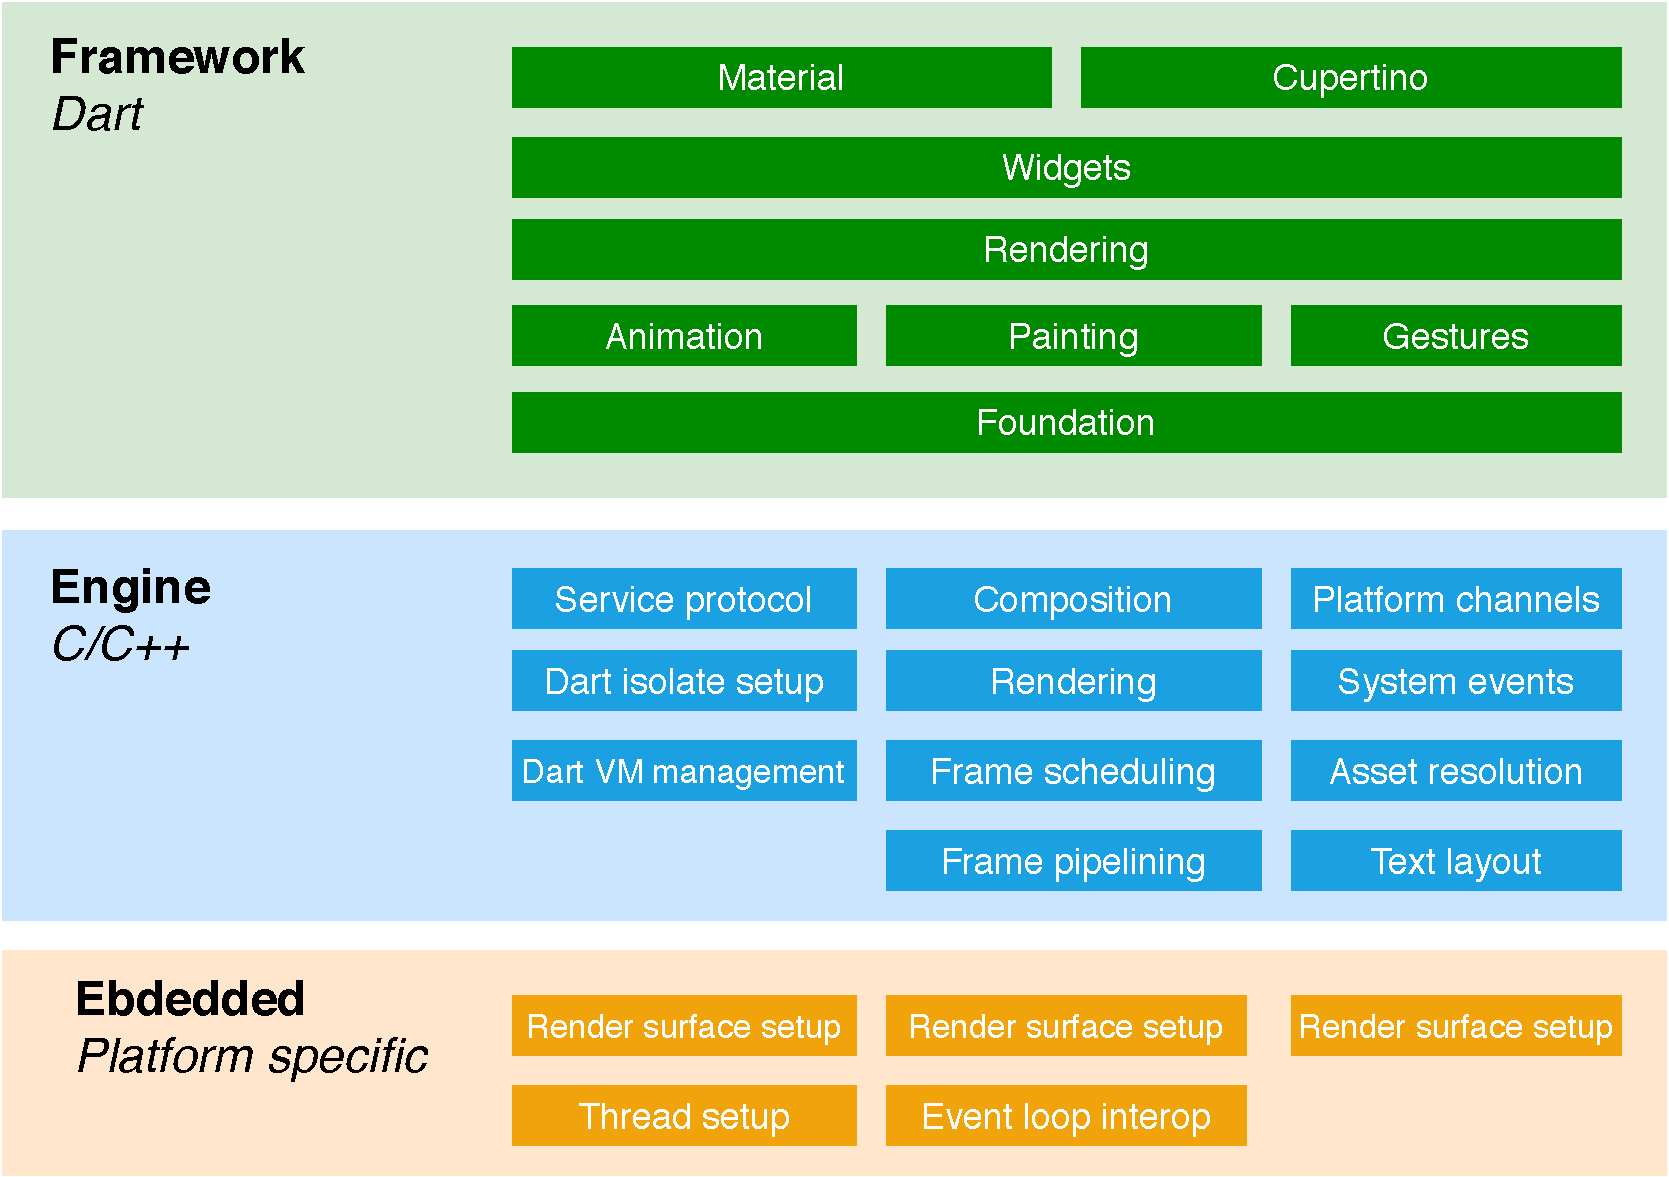
\includegraphics[width=\linewidth]{assets/technology-research/framework/flutter_overview.pdf}
    \caption{Vrstvy frameworku Flutter~\cite{flutter_technical_overview}}
    \label{fig:flutter_layers}
\end{figure}

Na obrázku~\ref{fig:flutter_layers} lze vidět uspořádání frameworku do vrstev
architektury.
Vrstva frameworku samotného je na úrovni widgetů,
které píší vývojáři aplikací v jazyce Dart.
Vrstva enginu ovládá framework na nižší urovni, kompozici widgetů,
jejich vykreslování a podobně.
Engine je vyvíjen v programovacích jazycích C a C++.
A vrstvě zaměřené na požadavky specifické
platformy.~\cite{flutter_technical_overview}

Pokud se widget potřebuje měnit na základě dynamických faktorů,
jako je například interakce uživatele nebo tok dat,
je tento widget označován jako \emph{stateful} (widget se stavem) a je
reprezentovaný třídou \mintinline{dart}|StatefulWidget|.
V opačném případě je widget označován jako \emph{stateless} a je 
reprezentovaný třídou \mintinline{dart}|StatelessWidget|,
která má stav neměnný.
Každý stateful widget má proměnlivý stav \mintinline{dart}|State|
a kdykoli je stav změněn,
je potřeba zavolat metodu \mintinline{dart}|setState()|,
která signalizuje frameworku,
že je widget nutno překreslit s novým stavem.~\cite{flutter_technical_overview}

\subsubsection*{Další platformy}

Framework Flutter momentálně vyvíjí také podporu pro
další platformy jako jsou platformy web a desktop.
Tyto platformy jsou zatím podporovány pro produkci,
avšak dle obrázku~\ref{fig:flutter_layers_web} lze vidět,
že framework Flutter je navržen vhodně k tomu,
aby tato a další úsilí podpořil.
Spodní specifické vrstvy platformy jsou vyměněny za vykreslování pomocí
webových technologií,
což v budoucnu umožní vytvářet aplikace nejen pro platformy Android a iOS,
ale i již zmíněný web a desktop.~\cite{flutter_web, flutter_desktop} 

\begin{figure}[ht!]
    \centering
    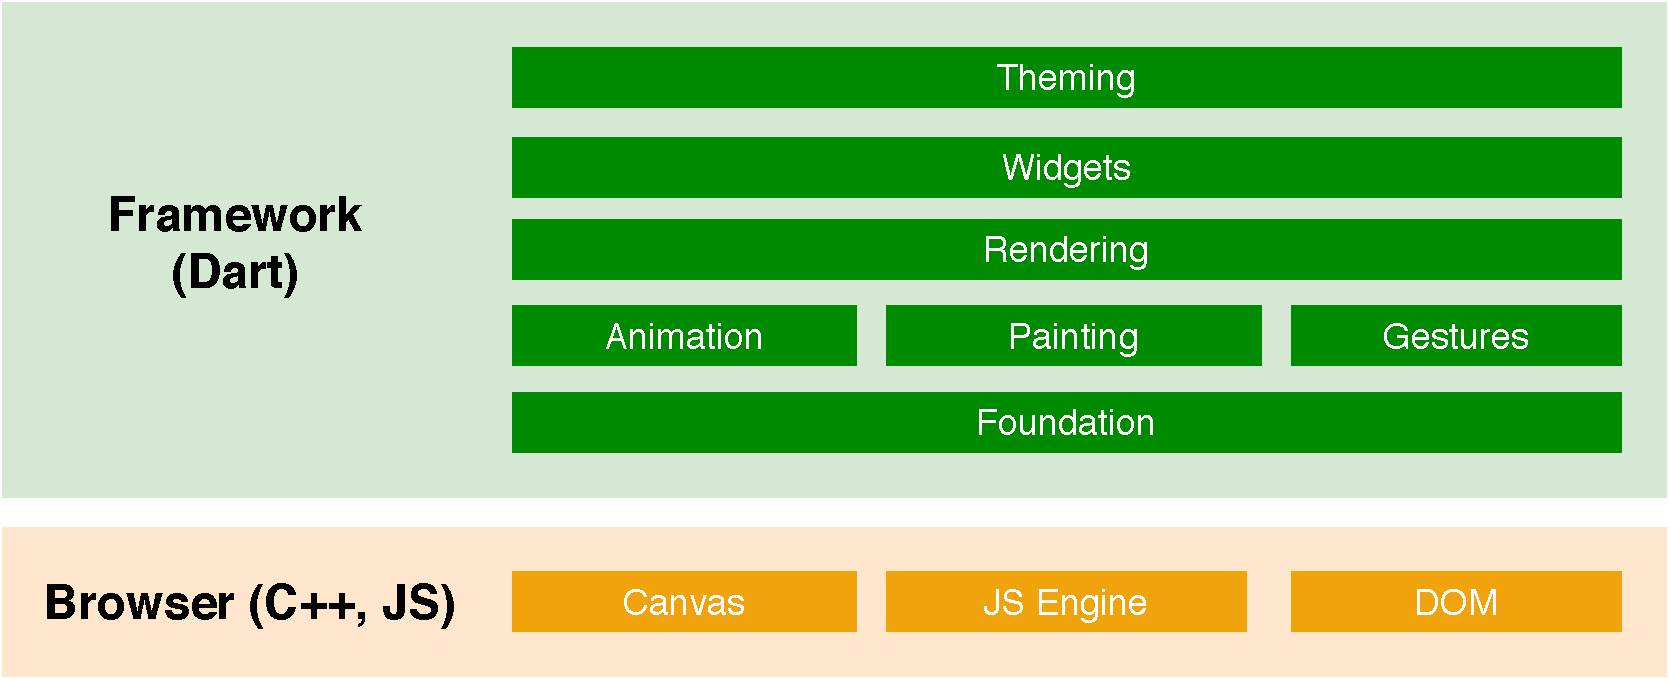
\includegraphics[width=\linewidth]{assets/technology-research/framework/flutter_overview_web.pdf}
    \caption{Vrstvy frameworku Flutter pro platformu web~\cite{flutter_web}}
    \label{fig:flutter_layers_web}
\end{figure}

\subsection{Zhodnocení}

Jak je již vidět z obrázku~\ref{fig:framework_popularity},
nejpopulárnější multiplatformní frameworky jsou frameworky Flutter a
React Native.
Přičemž framework Flutter je v porovnání s frameworkem React Native relativně
stále nový.
I přes to má ale dlouhodobě strmější růst v trendu.

Trend frameworku Ionic dlouhodobě stagnuje, až klesá,
a navíc kvůli již zmiňovaným nevýhodám,
zejména díky architektuře,
není až tolik vhodný pro vývoj nových aplikací,
s předpokladem pro dlouhodobější udržitelnost. 

Framework React Native je velmi populární a nabízí skvělé výhody.
Tento framework je však moc spjat s webovými technologiemi
a je nutné využívat komunikační most,
což přináší menší rychlostní i výkonostní nevýhody.
Framework Flutter oproti tomu přináší spoustu výhod,
a jak lze vidět z obrázku~\ref{fig:framework_flutter},
tak také zaručuje svou architekturou stejné zobrazení aplikace na všech
verzích operačních systémů dané platformy,
díky vlastnímu vykreslování.
Oba frameworky jsou zajisté vhodné pro vývoj nové aplikace s důrazem na
udržitelnost a rozšiřitelnost,
avšak framework Flutter převyšuje svými výhodami,
a proto bude v praktické části práce využit právě framework Flutter.

%https://github.com/tenhobi/bachelors-thesis/issues/14
% jak funguje stav v aplikaci; rozdíl mezi UI a APP stavem;
% jak řeší state management jednotlivé možnosti
\section{State management}

TODO text.

https://www.didierboelens.com/2019/04/bloc---scopedmodel---redux---comparison/

https://github.com/devonfw-forge/devonfw4flutter/wiki/200-Architecting-a-Flutter-App

https://flutter.dev/docs/development/data-and-backend/state-mgmt/declarative

https://flutter.dev/docs/development/data-and-backend/state-mgmt/intro

%\subsection{Ephemeral vs. App}

2 druhy stavů.

\begin{description}
    \item[Ephemeral state] describing text
    \item[App state] describing text
\end{description}

Jak se liší. Je to tohle nebo tamto? 

https://flutter.dev/docs/development/data-and-backend/state-mgmt/intro

https://flutter.dev/docs/development/data-and-backend/state-mgmt/ephemeral-vs-app

https://flutter.dev/docs/development/data-and-backend/state-mgmt/options

\subsection{Provider}

TODO text.

\subsection{Redux}

TODO text.

\subsection{BLoC}

TODO text.

%https://github.com/brianegan/flutter_architecture_samples/tree/master/bloc_library

\subsubsection{Implementace Felixe Angelova}

TODO text.

\subsection{Zhodnocení}

TODO text.

\section{Databáze}

Aby aplikace mohla uchovávat data napříč aplikacemi,
musí využívat některé databázové řešení.
Databáze je souhrn informací,
které jsou vhodně uspořádány tak,
že jsou snadno dostupné a udržovatelné.
Oproti jednomuchému ukládání dat do souboru na disku mají databáze hodně výhod.
Data lze vyhledávat pomocí speciálních dotazů,
lze je slučovat pomocí spojovacích funkcí,
jsou tolerantní k chybám
a může je používat vícero uživatelů najednou.
A to všechno při zachování optimální rychlosti.
\cite{database}

Dle~\cite{sql_nosql} existuje několik typů databází a přístupů k datům,
přičemž největší rozdíly jsou v tom,
jak ukládají který typ dat,
a jak je k těmto datům umožněno přistupovat.
\todo{\emph{\uv{Relational databases are structured,
while non-relational databases are document-oriented and distributed.}}}
\cite{sql_nosql}

Zatímco Structured Query Language (dále jen SQL) databáze byly donedávna
preferovaným způsobem databází~\cite{sql_nosql},
trendem posledních let jsou Non SQL (dále jen NoSQL) databáze.
Popis těchto typů databází,
včetně výhod a nevýhod jednotlivého řešení,
je shrnuto v následujících sekcích.

\subsection{SQL}

Data v SQL databázích jsou ukládány strukturovaně,
čímž tyto databáze dosáhnout největších výhod.
Výhodou také je jejich široká podpora a snadné řešení chyb.
Principem těchto databází jsou vlastnosti,
které shrnuje ACID (atomičnost, koexistence, izolace, trvanlivost).
Těmito vlastnostmi databáze redukuje anomálie a chyby způsobené transakcemi.
Díky dlouhé době,
za kterou se SQL databáze již používali,
existuje spousta nástrojů a doplňků,
které usnadňují vývoj a řešení případných chyb.
Nevýhodou je však náročnější škálování databáze při vývoji aplikace.
Příkladem je například databáze MySQL.
\cite{sql_nosql}

\subsection{NoSQL}

Data v NoSQL databázích jsou většinou nestruktorovány.
Tím získávají tyto databáze velký náskok co se flexibility dat a rychlosti
přístupu týče.
Tyto databáze je vhodné vnímat především jako klekce,
které obashují dokumenty. 
NoSQL databáze jsou vhodné pro ukládání velkého množství nestruktorovaných dat,
u kterých není nutné předem definovat jejich podobu.
Nevýhodou je však relativní novost tohoto přístupu,
což znamená i menší počet nástrojů,
jako jsou nástroje k analýze a řešení problémů.
Tyto databáze většinou používají vlastní dotazovací jazyk či jiné standardizace,
což může vést k problémům při přechodu na jinou databázi.
\cite{sql_nosql}
Příkladem je například databáze Cloud Firestore.
\cite{cloud_firestore}

\subsection{Firebase: Cloud Firestore}

Firebase je projekt,
který pomáhá vývojářům s mobilními a webovými aplikacemi.
Díky Firebase mohou být aplikace tvořeny rychleji,
bez času stráveného budováním funkcionalit jako analytika a databáze.
Tyto produkty jsou tvořeny na Google infrastruktuře
a jsou využívány společnostmi jako jsou The New York Times,
Duolingo, Alibaba, \dots{}
\cite{firebase}

Cloud Firestore je flexibilní NoSQL databáze dostupná v projektu Firebase.
Tato databáze lehce spolupracuje s ostatními produkty Firebase,
jako jsou autentikace, správa práv nebo automatické aktualizace dat.
Spolu s databází je poskytována řada balíčků pro vývoj mobilních a webových
aplikací,
které poskytují přátelské rozhraní k vývoji s touto databází.
Dostupná je také funkce offline podpory,
která automaticky ukládá často používané data,
které je možno používat i bez internetového spojení.
Data je možné filtrovat pomocí speciálních dotazů na kolekce i dokumenty
a je možné také tyto dotazy kombinovat a řadit.
\cite{cloud_firestore}

\subsection{Zhodnocení}

Vývoj herní aplikace je ideální pro využití NoSQL databází.
V takovéto aplikaci se najde plno příležitostí,
kde lze využít rysů těchto databází,
kde by naopak rysy SQL databází působily zbytečné obtíže.
I když nedisponují ACID vlastnostmi,
je využití tohodo typu databáze,
konkrétně databáze Cloud Firestore,
nejvhodnější pro vývoj praktické části práce,
proto bude použita právě databáze Cloud Firestore.

\section{Senzory}

% https://developer.android.com/guide/topics/sensors/sensors_overview
% Motion Sensors
% Position Sensors
% Environment Sensors

% https://developer.android.com/guide/topics/sensors
% https://source.android.com/devices/sensors/sensor-types
% https://source.android.com/devices/sensors
% https://www.javatpoint.com/android-sensor-tutorial
% https://heartbeat.fritz.ai/sensors-in-android-215df2c618de

\todo{Popsat obecně senzory, k čemu slouží atp. Jaké má mobil senzory, jaké využiju (otáčení, třesení), ...}
\blind[2]

\subsection{\todo{První kapitola o nějakém senzoru.}}

\blind[2]

\subsection{\todo{Druhá kapitola o nějakém senzoru.}}

\blind[3]

\subsection{Zhodnocení}

\todo{Bude tu?}

\section{Architektura}

Stroje,
které sestavují či spouštejí aplikace,
nezajímá vzhled či uspořádání zdrojového kódu.
Naopak vývojáři,
jakožto lidé,
potřebují udržovat kód snadno čitelný a srozumitelně rozdělený do jednotlivých
motod, tříd, struktur či vrstev aplikace.
Potřebují také vysokoúrovňové jazyky či pokročilé knihovny a frameworky,
které ulehčí psaní kódu a nenutí vývojáře psát vše odznovu.
I přes to ale nejsou aplikace psány dle nejlepších doporučení
a velmi často vývojáři píší či naráží na tak zvaný \uv{spaghetti code}.
To je mnohdy zapříčeněno nárokem na rychlou implementaci nových funkcí či úprav,
kde vývojáři na úkor času zanedbají čitelnost a strukturu kódu
a čím dál tím více postupem času prohlubují dluh kvality daného kódu.
\cite{architecture}
\todo{\emph{\uv{Software has two types of value:
the value of its behavior and the value of its structure.
The second of these is the greater of the two
because it is this value that makes software soft.}}}
\cite{martin_clean_architecture}
\todo{Jak odkazovat na přímou citaci?}
Dle zmíněného zdroje také plyne,
že se dlouhodobě vyplatí vývoj směřovat k dobré struktuře a architektuře,
než k samotné implementaci,
jelikož implementace se snadno opraví,
kdežto opravit architekturu bez velkého zásahu je značně obtížné.
\cite{martin_clean_architecture}

Cílem každé aplikace je mít udržitelný a snadno rozšiřitelný kód.
Je proto třeba stanovit řadu pravidel,
které pomohou s vývojovými otázkami při návrhu metod, tříd, rozhraní či
celých modulů.
Architektura a její správný a promyšlený návrh umožňuje vyvarovat
se chyb a dluhu ve formě kvality a modularity,
který znemožní snadný proces udržitelnosti aplikace.
\todo{\emph{\uv{Good architecture makes the system easy to understand,
easy to develop, easy to maintain, and easy to deploy.
The ultimate goal is to minimize the lifetime cost of the system
and to maximize programmer productivity.}}}
\cite{martin_clean_architecture}
Dobře navržená a udržovaná architektura tak umožní z dlouhodobého hlediska
produkovat kvalitnější kód.
Kvalitnější architektura tedy logicky minimalizuje nutnost oprav a
přizpůsobení struktury aplikace při vývoji každé nové funkcionality.

Dle zdroje~\cite{architecture} lze rozdělit architektury do dvou skupin:
architektury zaměřené na databázi a architektury zaměřené na doménu.
V následujících sekcích budou popsány rozdíli mezi oběmi skupinami
a vybrané konkrétní případy architektur.

\subsection{Architektury zaměřené na databázi}

Architektury zaměřené na databázi,
také nazývané \emph{database-centric architectures},
byly dle~\cite{architecture} prvním typem softwarových architektur.
Tyto architektury staví databáze do středu dění,
jak jde vidět z obrázku~\ref{fig:architecture_database}.

\begin{figure}
    \centering
    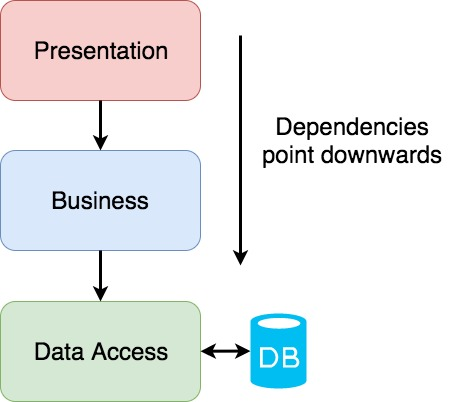
\includegraphics[width=0.5\linewidth]{assets/technology-research/architecture/database-centric.jpg}
    \caption{Schéma architektury zaměřené na databázi \todo{do vektoru}~\cite{architecture}}
    \label{fig:architecture_database}
\end{figure}

Příkladem tohoto typu architektury je tradiční 3-vrstvá architektura.
Ta je robustní a škálovatelná.
Skládá se ze tří vrstev.
První vrstva,
prezentační vrstva,
obsahuje tvorbu UI,
bez samotného kódu s logikou.
Druhá vrstva,
aplikační vrstva,
obsahuje samotné kód s logikou.
Tato vrstva by měla být nezávislá na prezentační vrstvě,
avšak má explicitní závislost na datové vrstvě.
Poslední vrstva,
datová vrstva,
je nejspodnější vrstvou,
která se stará o manipulaci a tok dat z databáze do nižších vrstev.
\cite{architecture}

\begin{listing}
    \caption{Ukázka přístupu zaměřeného na databázi v jazyce Java~\cite{architecture}}
    \label{code:architecture-database}
    \begin{minted}{java}
package ua.com.crosp.testapp.domain;
import ua.com.crosp.testapp.datalayer.PostsRepository;

public class GetRecentPostsUseCase
implements GetRecentPostsUseCaseContract {
    private PostsRepository mPostsRepository;

    public Single<Post.List> execute(Params params) {
        // Execute
    }
}
    \end{minted}
\end{listing}

V této architektuře je největší role přikládána databázi
a často je tak datová a aplikační vrstva úzce propojena.
V nejhorších případech na datové vrstvě závisí i vrstva prezentační.
\cite{architecture}
Ukázka přístupu pomocí této architektury je znázorněna ve výpisu kódu
\ref{code:architecture-database}.

\subsection{Architektury zaměřené na doménu}

\begin{figure}
    \centering
    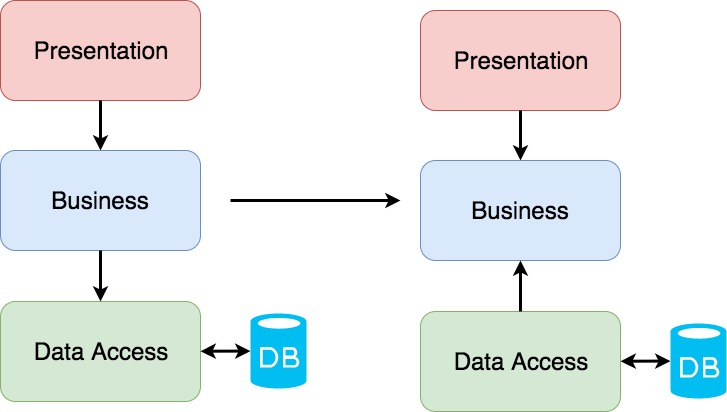
\includegraphics[width=0.5\linewidth]{assets/technology-research/architecture/domain-centric.jpeg}
    \caption{Schéma architektury zaměřené na doménu \todo{do vektoru; oříznout?}~\cite{architecture}}
    \label{fig:architecture_domain}
\end{figure}

Architektury zaměřené na doménu,
také nazývané \emph{domain-centric architectures},
je produktem vývoje z předchozího typu architektur.
Střed dění je přesunut na aplikační vrstvu
--- jak jde vidět z obrázku~\ref{fig:architecture_domain} ---,
protože právě tato vrstva je v aplikaci nejdůležitější,
jelikož se v ní děje implementace nových funkcionalit, změn či oprav.
\cite{architecture}
\todo{\emph{\uv{The way you keep software soft is
to leave as many options open as possible,
for as long as possible.
What are the options that we need to leave open?
They are the details that don’t matter.}}}
\cite{martin_clean_architecture}
Výhodou architektur zaměřených na doménu tedy také je,
že již díky návrhu samotnému abstrahují implementační detaily do podoby
kontraktů.
Těmto kontraktům může nadále vyhovět několik konkrétních implementací,
což umožní snadnou výměnu služeb či jiných závislostí.
\cite{martin_clean_architecture}
Lze tak tedy jednoduše nahradit třeba konkrétní databázi
--- například z databáze MySQL na databázi Cloud Firestore ---,
bez toho,
aniž by se muselo zasahovat do samotné aplikační vrstvy aplikace.
Ukázka přístupu pomocí tohoto typu architektury je znázorněna ve výpisu kódu
\ref{code:architecture-domain}.

\begin{listing}
    \caption{Ukázka přístupu zaměřeného na doménu v jazyce Java~\cite{architecture}}
    \label{code:architecture-domain}
    \begin{minted}{java}
package ua.com.crosp.testapp.domain;
import ua.com.crosp.testapp.domain.PostsRepositoryContract;

public class GetRecentPostsUseCase
implements GetRecentPostsUseCaseContract {
    private PostsRepositoryContract mPostsRepository;

    @Inject
    public GetRecentPostsUseCase(PostsRepositoryContract r) {
        mPostsRepository = r;
    }
    public Single<Post.List> execute(Params params) {
        // Execute
    }
}
    \end{minted}
\end{listing}

\subsection{Clean Architecture}

\todo{Dokončit kapitolu o CA.}

\todo{\emph{\uv{Good software systems begin with clean code.
On the one hand, if the bricks aren’t well made,
the architecture of the building doesn’t matter much.
On the other hand, you can make a substantial mess with well-made bricks.
This is where the SOLID principles come in.}}}~\cite{martin_clean_architecture}

%https://gist.github.com/ygrenzinger/14812a56b9221c9feca0b3621518635b

\todo{Co je Clean Architecture~\cite{martin_clean_architecture}, proč je to fajn používat atp.}
\blind{3}
 
%https://hackernoon.com/hammering-at-clean-architecture-1wbr3cgo

%https://github.com/ResoCoder/flutter-tdd-clean-architecture-course

%https://stackoverflow.com/questions/23479879/clean-architecture-vs-onion-architecture

%TOHLE !! https://crosp.net/blog/software-architecture/clean-architecture-part-2-the-clean-architecture/

%https://blog.cleancoder.com/uncle-bob/2012/08/13/the-clean-architecture.html

%https://github.com/android10/Android-CleanArchitecture

%https://dev.to/bosepchuk/why-i-cant-recommend-clean-architecture-by-robert-c-martin-ofd

%https://proandroiddev.com/clean-architecture-data-flow-dependency-rule-615ffdd79e29

%https://www.freecodecamp.org/news/a-quick-introduction-to-clean-architecture-990c014448d2/

%https://proandroiddev.com/multiple-ways-of-defining-clean-architecture-layers-bbb70afa5d4a

%https://github.com/bufferapp/android-clean-architecture-boilerplate

% https://github.com/bufferapp/android-clean-architecture-boilerplate

\subsection{Zhodnocení}

\todo{Popsat proč si vybírám Clean Architecture.}
\blind{1}

\section{Testování}

Testování se v průběhu let stalo nedílnou součástí vývoje aplikací.
Je vhodné pro všechny velikostí aplikací,
především proto,
že testování vede k vyšší kvalitě kódu \cite{testing_quality}
a tím k snadnější udržitelnosti aplikace.
Cílem testů je ověřit a dále kontrolovat,
že specifické části aplikace fungují
a že zachovávají tuto funkčnost při jejich úpravě.
Této podkapitole jsou popsány typy testů, vzory a přístupy,
které pomáhají k snažšímu testování.

\subsection{Typy testů}

Testovat je možné i ručně.
To však je však z globálního hlediska neefektivní a zdlouhavé.
V praxi se proto využívají automatizované testy,
které lze spustit samostatně kdykoli během cyklu vývoje aplikace.
Dle \cite{testing_flutter} se automatizované testy dělí do těchto kategorií:

\begin{description}
    \item[Unit testy] Testují jednu funkci, metodu nebo třídu.
    Tento typ testů je snadné vytvořit,
    rychle se spouští
    a jejich smyslem je ověřit správnou funkčnost dané části.
    Externí závislosti jsou nahrazeny jejich testovací kopií,
    která neprovádí žádnou funkčnost.
    \item[Widget testy] Někdy také nazývané jako \emph{component testy},
    testují jeden widget jako celek.
    Jejich smyslem je ověřit,
    jestli se daný widget chová a vypadá dle očekávání.
    Tento typ testů je složitější vytvořit a udržovat.
    \item[Integrační testy] Testují celou aplikaci nebo její části.
    Tento typ testů je složité vytvořit,
    mají velké množství závislostí a jsou velmi pomalé na spuštění.
    Na druhou stranu testují korektnost aplikace,
    či její části,
    jako celku.
\end{description}

Ve výpisu kódu \ref{code:test-unit} lze vidět příklad unit testu.
\cite{testing_flutter_unit}
Unit testování vyžaduje jako závislost pro vývoj balíček
\mintinline{dart}|test|.
Příklad obsahuje čítač reprezentovaný třídou \mintinline{dart}|Counter|,
která umí svou hodnotu \mintinline{dart}|value| inkrementovat pomocí
metody \mintinline{dart}|increment()|.
Jak lze vidět,
použitý balíček umožní vývojáři využívat například metody
\mintinline{dart}|test()| a \mintinline{dart}|expect()|,
díky kterým lze popsat očekávaný stav každého testu.

Ve výpisu kódu \ref{code:test-widget} lze naopak vidět příklad widget testu.
\cite{testing_flutter_widget}
Testování widgetů vyžaduje jako závislost pro vývoj balíček
\mintinline{dart}|flutter_test|.
Příklad ukazuje ukázku toho,
jak lze u testovaného widgetu otestovat očekávané položky \emph{title}
a \emph{message}.
Princip funkčnosti je stejný,
jako u balíčku \mintinline{dart}|test|,
jen se namísto metody \mintinline{dart}|test()|
využívá metoda \mintinline{dart}|testWidgets()|.

\begin{listing}
    \caption{Ukázka unit testu \cite{testing_flutter_unit}}
    \label{code:test-unit}
    \begin{minted}{dart}
        import 'package:test/test.dart';
        import 'package:counter_app/counter.dart';
        
        void main() {
          test('Counter value should be incremented', () {
            final counter = Counter();
        
            counter.increment();
        
            expect(counter.value, 1);
          });
        }
    \end{minted}
\end{listing}

\begin{listing}
    \caption{Ukázka widget testu \cite{testing_flutter_widget}}
    \label{code:test-widget}
    \begin{minted}{dart}
    import 'package:flutter/material.dart';
    import 'package:flutter_test/flutter_test.dart';

    void main() {
        testWidgets(
            'MyWidget has a title and message',
            (WidgetTester tester) async {
            await tester.pumpWidget(MyWidget(title: 'T', message: 'M'));

            final titleFinder = find.text('T');
            final messageFinder = find.text('M');

            expect(titleFinder, findsOneWidget);
            expect(messageFinder, findsOneWidget);
            },
        );
    }
    \end{minted}
\end{listing}

\subsection{Code coverage}

Code coverage znamená pokrytí kódu.
V testování to je pojem,
který značí,
do jaké míry jsou třídy a jejich vlastnosti a metody otestovány.
Určitě ale neplatí,
že 100 \% code coverage značí,
že je aplikace správně otestována.
Tato metoda identifikuje kód,
který již není používán,
nebo ani nikdy nebyl,
nebo dokonce netestovatelný kód,
způsobený špatnou implementací.
\cite{code_coverage}

Code coverage také monituruje vývoj v čase,
případně popisuje změny,
které by se do aplikace zanesli při připojení kódu ve verzovacím systému.
V rámci systémů rozšiřující verzovací systém lze využívat několik nástrojů,
které code coverage
--- v rámci kontinuální integrace, která je popsána v kapitole \ref{chap:ci} ---
moniturují a podávají vývojářům zprávy.
Příkladem těchto služeb může být CodeCov či Coveralls.
Každý soubor či složka je ohodnocen procenty,
které značí poměr otestovaného a neotestovaného kódu.
Služba pracující s code coverage při každé obdržené dávce kódu spustí
průzkum kódu aplikace a porovná jej se stávající verzí.
\cite{code_coverage}

\subsection{Test driven development}

\emph{Test driven development} (dále jen TDD) je metoda pro vývoj aplikací tím
způsobem,
že se začíná psaním testů,
které je následováno psaním produkčního kódu,
které testy splňuje.
Dle \cite{tdd} má TDD tři jednoduchá pravidla:

\begin{enumerate}
    \item Není dovoleno psát žádný produkční kód kromě toho,
    který opravuje selhávající test.
    \item Není dovoleno psát více unit testů než je dostačující k selhání;
    a selhání kvůli kompilaci jsou také selhání.
    \item Není dovoleno psát více produkčního kódu,
    než je dostatečné pro úspěšné provedení unit testu.
\end{enumerate}

Nejdříve je tedy napsán unit test pro funkcionalitu,
kterou chce vývojář přidat.
Následně vývojář napíše jen tolik kódu,
kolik je třeba k opravě daného testu.
A celý proces se znovu opakuje.
Celá myšlenka \cite{tdd} stojí tedy na tom,
že mohu psát pouze kód,
který opravuje selhávající test.
Tento proces se zdánlivě zdá \uv{hloupý} a pomalý.
\emph{\uv{Přemýšlejte však o tom, co by se stalo, kdybyste vešli do místnosti plné lidí pracujících tímto způsobem. Vyberte libovolnou náhodnou osobu v libovolnou dobu. Před minutou fungoval celý její kód.}} \cite{tdd} (překlad vlastní)

Jak již bylo zmíněno,
dle výzkumu \cite{testing_quality} je navíc tento přístup velmi efektivní,
jelikož vede k vyšší kvalitě kódu.
Navíc,
dodržováním těchto tří pravidel přesně víme,
jak volat určité rozhraní,
jelikož pro to máme test.
Kdokoli potřebuje znát cokoli aplikaci,
existuje test,
který tuto činnost popisuje.
\cite{tdd}

\subsection{Kontinuální integrace}
\label{chap:ci}

Jakákoli aplikace se běžně skládá z mnoha částí
a obsahuje mnoho řádků kódu,
zatímco do sebe musí vše dokonale zapadat
a i nejmenší chyba může způsobit selhání sestavení aplikace.
Při přidávání nových funkcionalit je proto velké riziko,
že aplikace obsahuje chybu.
Při snaze připojení změn pomocí nástrojů rozšiřující verzovací systémy
tak proto nastává příležistos pro CI,
které provede sestavení aplikace a spustí automatizované testy.
V tomto okamžiku dostane vývojář skrze rozšiřující aplikace indikaci,
zda-li změny kód rozbijí,
nebo zda aplikace zůstane v funkční.
\cite{ci}

Použití CI je výhodné především při práci s v týmu.
Právě díky zmíněným výhodám lze připojovat změny rychle a bez obav o zanesení
jinak skrytých chyb.
Tyto nástroje jsou buď zabudované do nástrojů rozšiřujících verzovací systémy
jako jsou GitHub a jejich GitHub Actions či GitLab a jejich GitLab CI,
nebo nezávislé nástroje,
jako jsou Travis CI či CircleCI.
\cite{ci}


\chapter{Analýza}
\label{chap:analysis}

\todo{Napsat pár úvodních vět o analýze.}
\blind[2]

\section{Popis hry}

Mobilní hra je laděna satiricky do prostředí jaderné elektrárny,
kterou musí uživatelé,
hráči hry v rozdílných rolích,
zachránit od zničení.
Hra se nazývá \emph{\myAppName}
a její děj se odehrává v neznámé jaderné elektrárně.
V této elektrárně má většina pracovníků dovolenou,
a proto jsou přítomni jen dva lidé,
technik a manažer.
Náhlý problém zapříčiní,
že mezi těmito pracovníky byla zablokována cesta,
a tak se tito dva zaměstnanci musí domluvit pouze hlasem
a zařídit opravu elektrárny.
Technik vidí všechny řídící prvky,
manažer vidí plány a manuály.
Jejich cílem je tak společnou spoluprací zabránit neštěstí v podobě exploze. 

Hra je členěna do několika kapitol
a každá kapitola obsahuje několik statických misí.
Mise jsou statické v tom významu,
kdy mají jasně přednastaveny prvky,
které mise obsahuje,
avšak mění se konkrétní jejich nastavení.
To zajištuje jak možnost znovuopakovatelnosti,
tak poměrování s ostatními hráči.

Každá mise,
a tedy konkrétní hra samotná,
obsahuje několik modulů,
které reprezentují určité řídící prvky elektrárny.
To mohou být nejrůznější tlačítka či přepínače,
ale i speciální moduly,
reprezentující prvky elektrárny,
které nelze vypnout či opravit a musí být periodicky kontrolovány,
jako pumpa dodávající chladící vodu do reaktoru.
Kromě modulů je potřeba ve hře okamžitě provádět akce,
které se zobrazí.
Akce jsou většinou jednorázové,
kdy stačí provést danou akci,
ale mohou být i na dělší dobu,
po kteoru musí hráči tuto akci dodržovat.

Konkrétní mise začíná po tom,
co jsou oba pracovníci připraveni,
a je stisknuto tlačítko \emph{AZ-5},
které by mělo zajistit rychlé odstavení reaktoru,
avšak z neznámého důvodu nefunguje.
Po skončení každé mise,
případně souhrnně za všechny odehráné hry,
jsou zobrazeny statistiky hry.
Statistiky po hře zobrazí uplynulý čas,
potřebný k opravě.
Souhrnné statistiky zobrazují procento,
reprezentující průměrný uplynulý čas potřebný k opravám
v porovnání s časy celkovými.

\subsection{Akce}

Akce jsou jakýmsi přerušením,
které hráči okamžitě vykonat.
Příkladem akce může být \emph{zatřeste zařízením} nebo
\emph{otočte zařízení obrazovkou k zemi},
kde význam jednotlivých akcí je zjevný z jeho názvu.
Speciální akce je nutné vykonávat po delší dobu,
takovým příkladem může být speciální akce
\emph{držte zařízení vodorovně se zemí, obrazovkou k zemi, po dobu 30 sekund}.
Speciální akce jsou využívány zejména v pokročilejších kapitolách,
jelikož mohou značně komplikovat hru.

\subsection{Modul A}

\todo{Popis modulu A}
\blind{1}

\subsection{Modul B}

\todo{Popis modulu B}
\blind{1}

\subsection{Modul C}

\todo{Popis modulu C}
\blind{1}

\section{Funkční požadavky}

Funkční požadavky popisují jednotlivé požadavky na funkcionalitu aplikace.
Z pohledu uživatelů aplikace popisují akce,
které může uživatel provést.
Jednotlivé funkční požadavky,
či jejich uskupení,
mohou tvořit jednotlivé nezávislé moduly aplikace.~\cite{fr_nfr}

\begin{enumerate}[label=\textbf{F\arabic*}, ref=F\arabic*]
    \myItem{Přihlášení}
Uživatel se bude moci do aplikace přihlásit, resp. registrovat,
pomocí účtu Google.
    \myItem{Informace o aplikaci}
Aplikace obsahuje obrazovku s informacemi o aplikaci,
včetně jména autora, verze, popisu a odkazu na projekt.
    \myItem{Vytvoření hry}
Přihlášený uživatel může vytvořit hru.
Součastně hráč nastaví misi ke hraní.
    \myItem{Připojení do hry}
Přihlášený uživatel se může připojit do hry pomocí kódu.
    \myItem{Spuštění hry}
Po potvrzení, že jsou hráči připraveni na hru,
mohou spustit hru s danou misí.
    \myItem{Ukončení hry}
Hráč může během přípravy hry nebo hraní hry danou hru ukončit.
    \myItem{Statistika po hře}
Hráčům je po skončení hry zobrazena herní statistika.
    \myItem{Zobrazení svého profilu}
Přihlášený uživatel si může zobrazit svůj profil.
    \myItem{Zobrazení svých statistik}
Přihlášený uživatel si může zobrazit své souhrné statistiky
ze všech hraných misí.
    \myItem{Změna nastavení}\label{req:settings}
Přihlášený uživatel si může změnit nastavení.
    \myItem{Odhlášení}\label{req:logout}
Přihlášený uživatel se bude moci z aplikace odhlásit.
\end{enumerate}

\section{Nefunkční požadavky}

\todo{Sem možná napsat nějaký info?}
\blind[1]

\begin{enumerate}[label=\textbf{N\arabic*}, ref=N\arabic*]
    \myItem{Multiplatformnost}
Aplikaci lze po nasazení spustit v současných verzích Android a iOS.
    \myItem{Udržitelnost a rozšiřitelnost}
Kód aplikace je psán přehledně,
s vhodnou architekturou a vhodnými konvencemi tak,
že je lehce udržitelný a rozšiřitelný.
    \myItem{Plynulost}
Aplikace funguje na všech obrazovkých plynule
i na výkonnostně slabších zařízeních.
    \myItem{Vícejazyčnost}
Aplikace podporuje češtinu a angličtinu
a je připravena na rozšíření o další jazyky.
\end{enumerate}

\let\oldsubsection=\thesubsection
\renewcommand\thesubsection{UC\arabic{subsection}} % UC* counter for subsections

\section{Případy užití}

Funkční a nefunkční požadavky sice definují funkcionalitu a vlastnosti aplikace,
avšak pro správné pochopení fungování a souhru těchto požadavků,
je nutné definovat případy užití,
které popisují jednotlivé problémy.
Případy užití jsou vytvořeny na základě stanovených funkčních požadavků,
s ohledem na stanovené nefunkční požadavky.

\subsection{Přihlášení}
\label{uc:login}

Tento případ užití popisuje proces přihlášení do aplikace.
Přihlášení probíhá pomocí účtu Google.
Proces zahrnuje i registraci,
pokud je uživatel v aplikaci nový.

\begin{enumerate}
    \item Uživatel klikne na tlačítko \emph{Přihlásit se}
    a následně proběhne přihlášení pomocí účtu Google.
    \item V závislosti na tom,
    jestli je uživatel již registrovaný,
    mohou nastat dvě situace:
    \begin{enumerate}
        \item pokud uživatel již byl registrovaný,
        je uživatel přihlášen a přesměrován na hlavní obrazovku;
        \item pokud uživatel ještě nebyl registrovaný,
        zobrazí se obrazovka,
        ve které vyplní své osobní údaje
        a následně je přihlášen a přesměrován na hlavní obrazovku.
    \end{enumerate}
\end{enumerate}

\subsection{Zobrazení informací o aplikaci}

Tento případ užití popisuje proces zobrazení informací o aplikaci.

\begin{enumerate}
    \item Uživatel se nachází na hlavní obrazovce a klikne na tlačítko
    \emph{O aplikaci}.
    \item Uživatel je přesměrován na obrazovku s informacemi o aplikaci,
    kde jsou zobrazeny informace jako jsou jméno vývojáře, verze aplikace,
    odkaz na repozitář se zdrojovým kódem nebo nejčastěji kladené otázky.
\end{enumerate}

\subsection{Změna nastavení}

Tento případ užití popisuje změnu nastavení,
kde lze zejména nastavit jazyk aplikace.

\begin{enumerate}
    \item Uživatel se nachází na hlavní obrazovce a klikne na tlačítko
    \emph{Nastavení}.
    \item Uživatel je přesměrován na obrazovku s nastavením.
    Zde může uživatel například přepínat jazyk aplikace.
\end{enumerate}

\subsection{Hra}

Tento případ užití popisuje proces vytvoření, spuštění a průběhu hry.
Případ užití je dělen do dvou scénářů.
První scénář popisuje uživatele,
který hru zakládá.
Druhý scénář popisuje uživatele,
který se do hry připojuje.

\subsubsection*{Scénář A -- zakládající uživatel}

Tento scénář popisuje případ užití pro uživatele,
který hru založí a hostuje.
Tento uživatel má také práva pro nastavení hry,
jako je kapitola a mise nebo role.

\begin{enumerate}
    \item Uživatel klikne na tlačítko \emph{Nová hra}
    a aplikace jej přesune na obrazovku místnosti.
    \item Zde uživatel vidí speciální kód,
    který předá spoluhráči.
    \item Uživatel vybere kapitolu,
    ve které vybere misi,
    a určí svou roli ve hře
    --- technik či navigátor.
    \item Uživatel klikne na tlačítko \emph{Připraven}.
    \item Až budou oba hráči připraveni ke hře,
    uživatel klikne na tlačítko \emph{AZ-5} a zahájí tak hru.
    \item Po skončení hry se uživateli zobrazí statistika ze hry.
\end{enumerate}

\subsubsection*{Scénář B -- připojující se uživatel}

Tento scénář popisuje případ užití pro uživatele,
který se připojuje do již vytvořené hry.
Tento uživatel nemá žádná práva pro nastavení.

\begin{enumerate}
    \item Uživatel klikne na tlačítko \emph{Připojit se}
    a aplikace jej přesuna na obrazovku místnosti,
    kde zadá kód hry.
    \item Uživatel klikne na tlačítko \emph{Připraven}.
    \item Po skončení hry se uživateli zobrazí statistika ze hry.
\end{enumerate}

\subsection{Ukončení hry}

Tento případ užití popisuje případy,
kdy a jak lze ukončit probíhající hru.

\subsubsection*{Scénář A -- dohrání}

Tento scénář popisuje standardní případ,
kdy hráč skončí hru dle předpokladů,
ať už úspěšně či neúspěšně.

\begin{enumerate}
    \item Uživatel se připojí do hry.
    \item Uživatel hraje hru.
    \item Uživatel dohraje hru, ať už úspěšně nebo neúspěšně.
    \item Aplikace zobrazí herní statistiky.
    \item Uživatel následně opustí hru kliknutím na tlačítko \emph{zpět}.
\end{enumerate}

\subsubsection*{Scénář B -- předčasné ukončení hry}

Tento scénář popisuje situaci,
kdy se jeden z hráčů rozhodne předčasně,
kvůli jakémukoli důvodu,
opustit hru a tím jí ukončit. 

\begin{enumerate}
    \item Uživatel se připojí do hry.
    \item Uživatel hraje hru.
    \item Uživatel klikne na tlačítko \emph{Ukončit hru}
    a potvrdí dialog.
    \item Aplikace zobrazí hlášku o předčasném ukončení hry.
\end{enumerate}

\subsection{Zobrazení profilu a statistik}

Tento případ užití popisuje,
jak uživatel zobrazí svůj profil a své souhrnné statistiky.

\begin{enumerate}
    \item Uživatel klikne na tlačítko \emph{Profil}.
    \item Aplikace zobrazí obrazovku profilu,
    která zobrazuje informace o profilu a souhrnné statistiky profilu.
\end{enumerate}

\let\thesubsection=\oldsubsection

\subsection{Přehled realizace požadavků}

Přehled realizace případů užití funkčními požadavky lze vidět v
tabulce~\ref{tab:use-case-requirements}.

\begin{table}[h!]
    \centering
    \begin{tabular}{c||c|c|c|c|c|c|c|c|c|c|c} 
        & F1 & F2 & F3 & F4 & F5 & F6 & F7 & F8 & F9 & F10 & F11 \\\hline\hline
        UC1 & X &   &   &   &   &   &   &   &   &   & X \\\hline % login logout
        UC2 &   & X &   &   &   &   &   &   &   &   &   \\\hline % info
        UC3 &   &   &   &   &   &   &   &   &   & X &   \\\hline % settings
        UC4 &   &   & X & X & X & X & X &   &   &   &   \\\hline % game
        UC5 &   &   &   &   &   & X &   &   &   &   &   \\\hline % game exit
        UC6 &   &   &   &   &   &   &   & X & X &   &   \\ % profile
    \end{tabular}
    \caption{Realizace případů užití a splnění požadavků}
    \label{tab:use-case-requirements}
\end{table}


\chapter{Návrh}

TODO text

\section{Uživatelské rozhraní}

Dle rešerše konkurenčních aplikací je cílem návrhu uživatelského rozhraní
vytvořit jednoduchou grafiku,
ve které se bude snadno navigovat a~kterou uživatel snadno pochopí.
Pro návrh uživatelského rozhraní je využíváno wireframů,
což je metoda pro návrh rozhraní,
kdy je obrazovka naskreslena pomocí jednoduchých tvarů
a~je tedy zobrazována struktura dané obrazovky,
místo konkrétního zpracování.
To slouží pro vyjádření základní reprezentace rozložení,
které ovšem nemusí být finální a~výsledná podoba obrazovek se může lišit. 
Veškeré wireframy byly vytvořeny pomocí programu draw.io.

V~následujících sekcích jsou popsány obrazovky jednotlivých modulů
s~obrázkami daných wireframů.

\subsection{Modul home}

Modul home slouží pro navigaci uživatele mimo hru samotnou.
Návrh tohoto modulu je velmi důležitý,
jelikož uživatele do samotné aplikace uvede a~umožní další postup.
Cílem návrhu tohoto rozhraní je snadno provést uživatele přihlášením,
registrací, menu, profilem, informacemi o~aplikaci a~nastavením.
Modul obsahuje celkem sedm obrazovek.

\begin{figure}
    \centering
    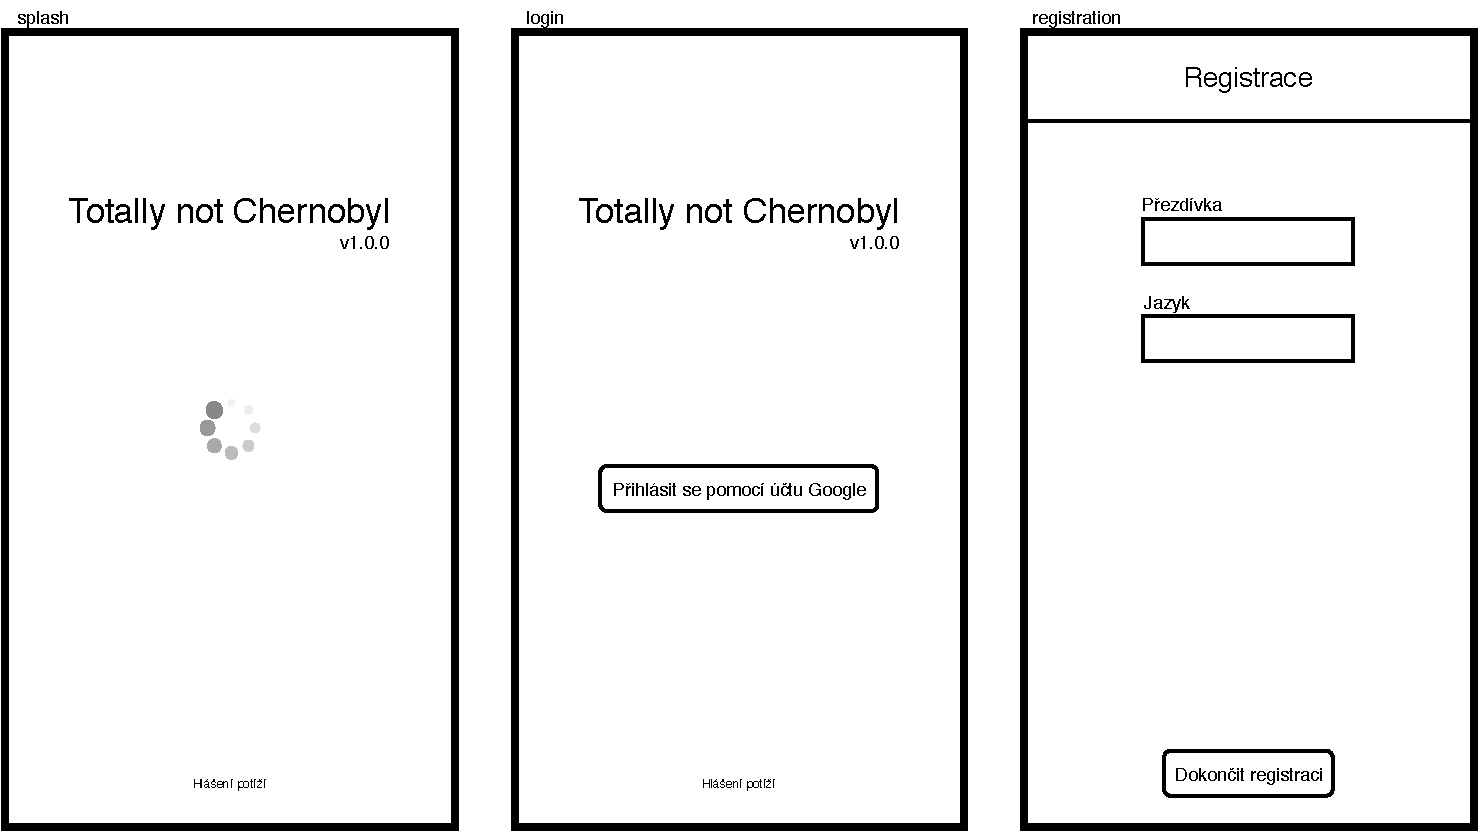
\includegraphics[width=1\linewidth]{assets/design/wireframes/home-1.pdf}
    \caption{Wireframy obrazovek splash, login a~registration}
    \label{fig:ui-home-1}
\end{figure}

Na obrázku~\ref{fig:ui-home-1} lze vidět obrazovky splash,
která slouží pro načítání aplikace,
login,
která slouží pro přihlášení uživatele,
a~registration,
která slouží pro vyplnění informací při registraci nového uživatele.
Tyto obrazovky jsou první,
které uživatel uvidí.
Proto je nutné,
aby byly obrazovky snadno pochopitelné a~jednoduché.
Uživatel na obrazovkách vidí pouze logo a~příslušné ovládací prvky,
což splňuje podmínky na jednoduchost.  

\begin{figure}
    \centering
    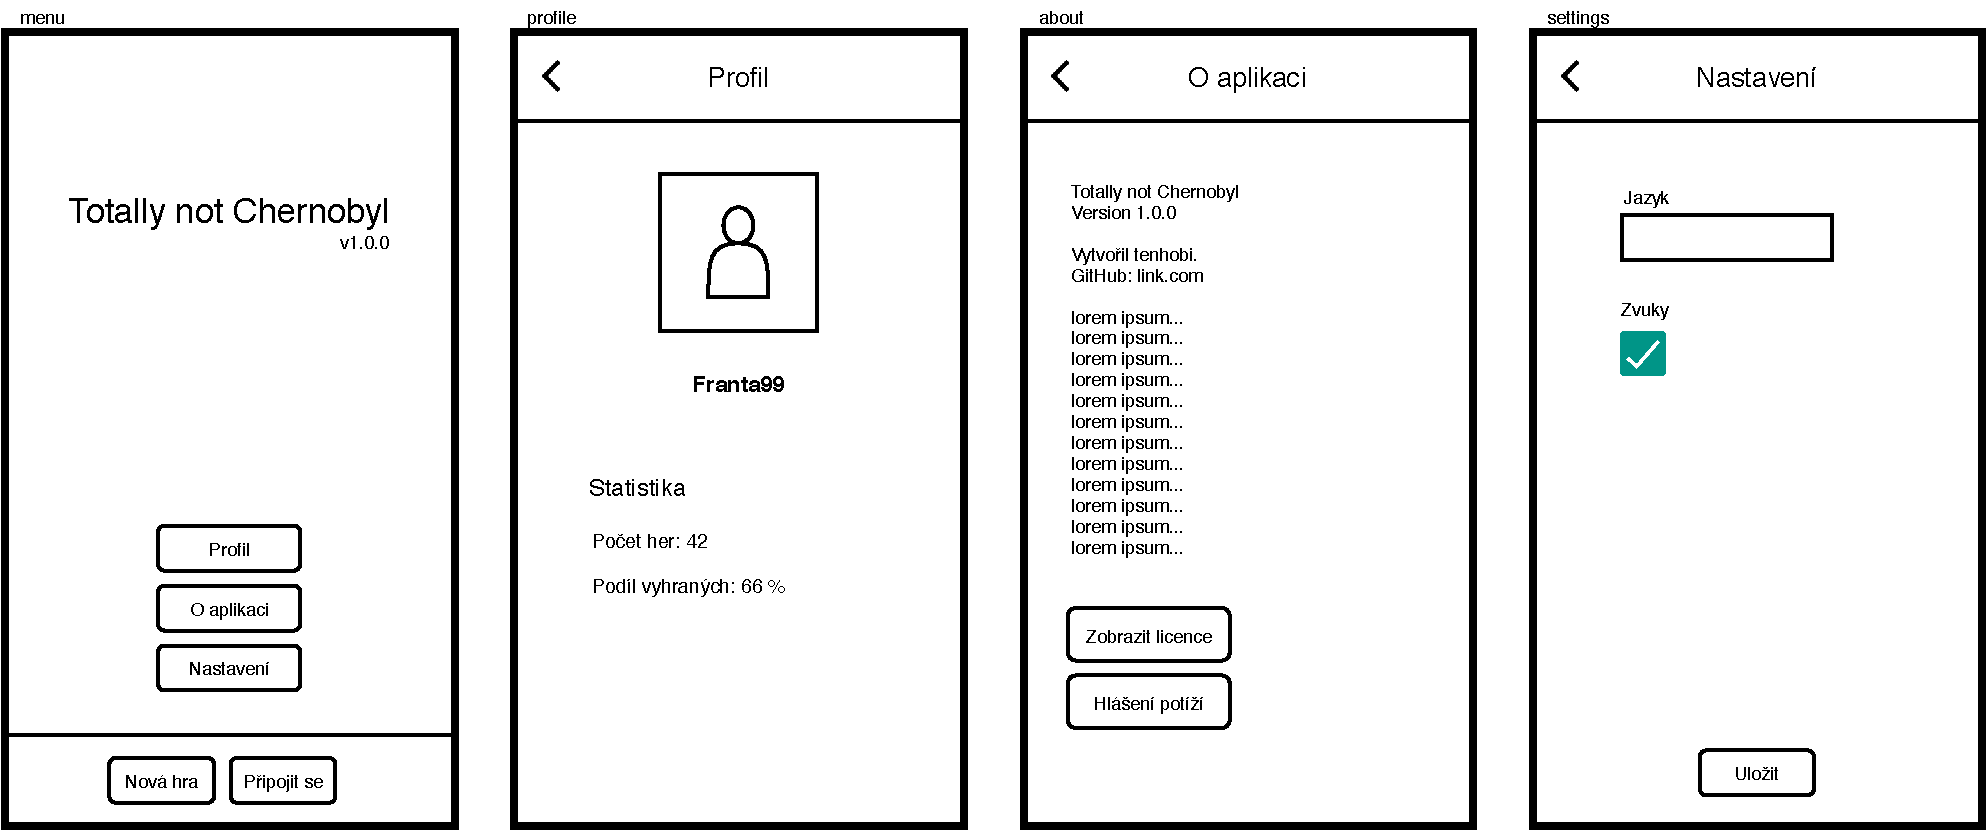
\includegraphics[width=1\linewidth]{assets/design/wireframes/home-2.pdf}
    \caption{Wireframy obrazovek menu, profile, about a~settings}
    \label{fig:ui-home-2}
\end{figure}

Po přihlášení do aplikace se uživatel přesune na obrazovku menu.
Z~této obrazovky se může uživatel přesunout kamkoli v~aplikaci,
a~proto jsou uživateli přehledně poskytnuta tlačítka,
která ho srozumitelně provedou.
Jedním z~nejdůležitějších tlačítek je vytvoření hry,
které je přehledně umístěno do spodní lišty.
Z~této obrazovky se uživatel může dostat na obrazovku profil,
kde jsou zobrazeny informace o~uživateli a~jeho statistiky.
Z~obrazovky menu se lze také prokliknout na obrazovky about a~settings.
Obrazovka about obsahuje informace o~aplikaci,
včetně názvu aplikace, verze, vývojáře a~tak podobně.
Na obrazovce settings může uživatel nastavit novou přezdívku nebo změnit jazyk
aplikace.
Tyto obrazovky lze vidět na obrázku~\ref{fig:ui-home-2}.

\subsection{Modul lobby}

Pro vytvoření hry se musí uživatel přesunout na obrazovky modulu lobby,
kde probíhá samotné nastavení hry před jejím vytvořením.
Na tyto obrazovky se dostane hráč z~modulu home po kliknutí na tlačítko
vytvoření hry nebo připojení se do hry.

\begin{figure}
    \centering
    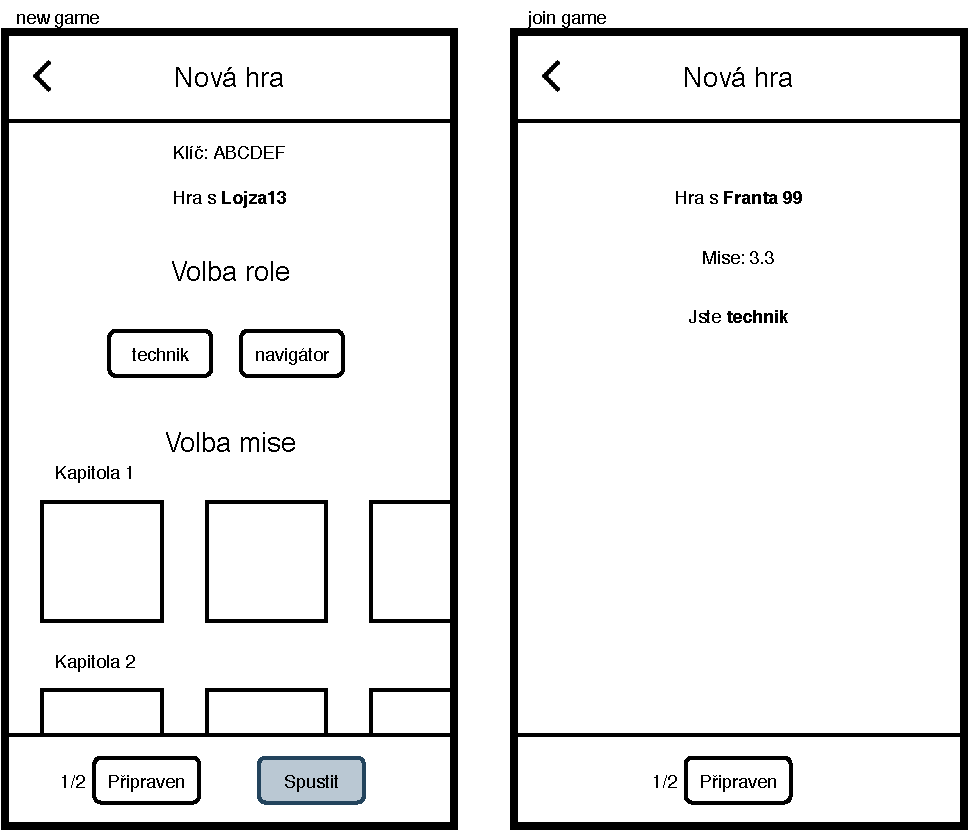
\includegraphics[width=0.6\linewidth]{assets/design/wireframes/lobby.pdf}
    \caption{Wireframy obrazovek new game a~join game}
    \label{fig:ui-lobby}
\end{figure}

\pagebreak
Na obrazovce new game může zakládající uživatel nastavit hru,
zejména si zvolit roli a~vybrat misi.
Na obrazovce uživatel vidí klíč pro připojení a~hráče,
který se do hry připojil.
Na dolní liště uživatel přehledně vidí tlačíko na signalizaci ke startu hry
a~k~odstartovánímu samotnému.
Na obrazovce join game vidí uživatel,
který se připojuje do hry,
pouze statické informace o~zvoleném nastavení.
Na dolní liště uživatel přehledně vidí tlačítko na signalizaci ke startu.
Tyto obrazovky jsou zobrazeny na obrázku~\ref{fig:ui-lobby}.

\subsection{Modul game}

Samotný modul hry je složen ze tří obrazovek.
Dvě obrazovky se věnují samotné hře a~zobrazují zbývající čas.
První obrazovka game manual slouží pro zobrazení informací ke vyřešení hry.
Druhá obrazovka je zajímavější.
Obsahuje samotné herní prvky,
mezi kterými musí hráč přepínat a~plnit je.
Třetí obrazovka je obrazovka po skončení hry,
která zobrazuje úspěch či neúspěch
a~statistiky hry.
Tyto obrazovky jsou vidět na obrázku~\ref{fig:ui-game}.

\begin{figure}
    \centering
    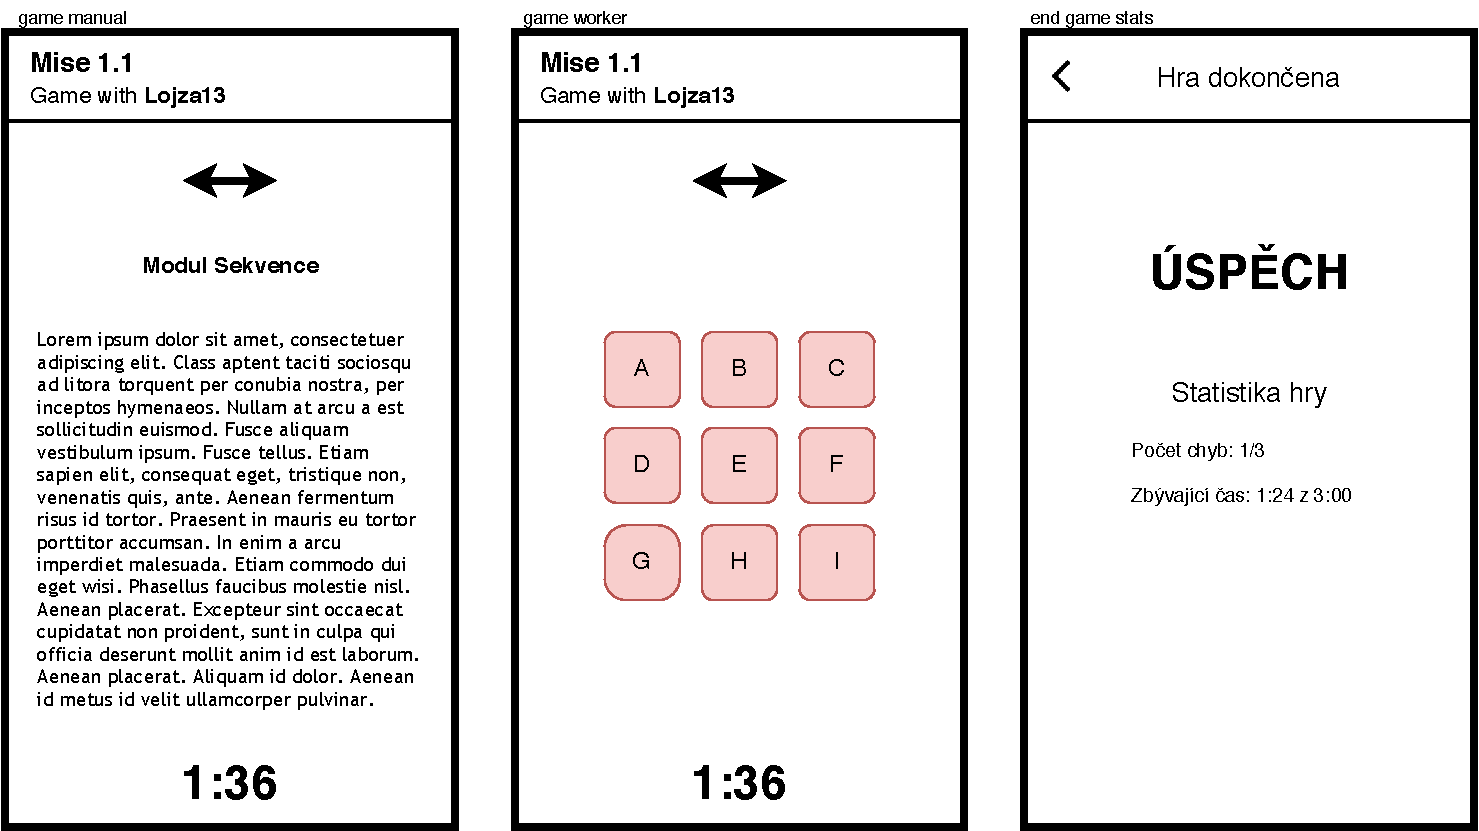
\includegraphics[width=1\linewidth]{assets/design/wireframes/game.pdf}
    \caption{Wireframy obrazovek game manual, game worker a~end game stats}
    \label{fig:ui-game}
\end{figure}

\section{Architektura}

\todo{Napsat o databázi, jak bude +- rozdělena na "event busy", které se budou starat o synchronizaci, resp. komunikaci, v rámci dané hry. Např. separátní pro akce hráčů, separátní pro úkoly atp.}

\todo{Pár úvodních slov o návrhu architektury.}
\blind{2}

\subsection{\todo{Možná návrh modulů/featur?}}

\todo{A pár slov a diagramů/grafů.}
\blind{2}

\subsection{\todo{Možná návrh hlavních struktur aplikace?}}

\todo{A pár slov a diagramů/grafů.}
\blind{4}

\subsection{\todo{Možná návrh zajimavých bloců?}}

\todo{A pár slov a diagramů/grafů.}
\blind{4}

\section{Lokalizace}

TODO text


\chapter{Implementace}
\label{chap:implementation}

Tato kapitola se zabývá popisem implementace aplikace.
V~následujících podkapitolách jsou popsány použité nástroje,
použité knihovny a~vybrané ukázky.
Aplikace byla implementována dle návrhu z~kapitoly~\ref{chap:design}.

\section{Použité nástroje}

Během vývoje byly použity nástroje,
které usnadnily vývoj aplikace či její ladění.
Pro samotné ladění aplikace byl využit nástroj \emph{scrcpy},
který umožní promítat obrazovku mobilního zařízení na obrazovku počítače
včetně bezdrátového spojení.

\begin{listing}
    \caption{Spuštění nástroje scrcpy pro bezdrátové použití}
    \label{code:scrcpy}
    \begin{minted}{shell}
adb tcpip 5555
adb connect DEVICE_IP:5555
scrcpy --window-title "Totally Not Chernobyl" --always-on-top
--bit-rate 2M --max-size 800
    \end{minted}
\end{listing}

\subsection{Verzování}

Během vývoje bylo využito verzovacích nástrojů.
To je běžná součást každého projektu a~slouží k~postupnému zaznamenávání změn.
V~této práci byl využit verzovací systém \emph{Git} a~webová služba \emph{GitHub},
která nabízí kromě bezplatného umístění repozitáře také doplňkové služby jako
code coverage, ticket systém, posouzení změn a~podobně.

\subsection{Editor}

Během vývoje aplikace byly využity dva editory.
Editor IntelliJ IDEA od společnosti JetBrains
a~editor VS Code od společnosti Microsoft.
Editor IntelliJ IDEA je robustní editor,
který obsahuje nápovědu a~analýzu kódu.
Díky výhodám jazyka Dart a~frameworku Flutter
byla však i~práce v~editoru VS Code snadná.
Pro oba editory jsou dostupné v~editorech chytré doplňky,
které využívají integrovaných nástrojů dodávaných s~jazykem Dart,
ale i~věci navíc jako poskytování útržků kódu pro usnadnění práce.

\section{Použité knihovny}

Při implementaci bylo využito několik knihoven,
které elegantně řeší dané specifické problémy.
Mezi nejzajímavější použité knihovny patří knihovny
\mintinline{Dart}|bloc| a~\mintinline{Dart}|flutter_bloc|,
které poskytují rozhraní knihovny a~widgety pro práci s~nimi.
Knihovna \mintinline{Dart}|easy_localization| řeší překlad uživatelského
rozhraní aplikace do několika jazyků.
Uživatel mezi jazyky může přepínat a~tím měnit jazyk prvků.
Lokalizace může být řešena více způsoby,
nejjednoduší a~jeden z~nejvíce efektivních je pomocí vytvoření několika souborů,
například ve formátu \mintinline{shell}|JSON| nebo \mintinline{shell}|YAML|,
které jednoduše a~přehledně umožní definovat slovník překladu.
Samotná definice ovšem ne vždy stačí.
Knihovna umožňuje vkládat parametry, které se do daného překladu vloží.
Knihovna \mintinline{Dart}|google_sign_in| poskytuje jednoduché rozhraní pro
přihlašování pomocí účtu Google.
Jelikož jazyk Dart nepodporuje třídy union,
knihovna \mintinline{Dart}|freezed| poskytuje rozhraní a~generátor pro
snadné generování těchto tříd.
Knihovna \mintinline{Dart}|url_launcher| umožní spouštění webových odkazů
nehledě na platformu.
Knihovna \mintinline{Dart}|cloud_firestore| poskytuje rozhraní k~práci se
stejnojmennou databází Cloud Firestore.
Dále je využito knihovny \mintinline{Dart}|effective_dart|,
která poskytuje souhrn pravidel pro statickou analýzu dle konvencí jazyka Dart.

\section{Dokumentace}

Z~implementace byla vytvořena také automatická vývojářská dokumentace.
Ta je ve formě webové stránky a~zobrazuje veřejné rozhraní tříd.
Komentáře jsou přehledně zobrazeny pomocí nástroje Markdown a~obsahují proklik
na třídy a~metody.
Tato dokumentace je umístěna na přiloženém datovém CD.

\section{Ukázky vybraných částí}

V~následujících sekcích je uvedeno několik ukázek z~implementace.
Každá ukázka reprezentuje určitou část vývoje a~popisuje její zajímavosti.

\subsection{Implementace widgetu}

V~ukázce kódu~\ref{code:implementation-1} je uvedena reprezentace implementace widgetu
ve frameworku Flutter.
Implementován je widget pro zobrazení loga aplikace.
Jedná se o~stateless widget,
což znamená,
že takovýto widget je zobrazen staticky a~nic se v~něm nemění.
Widget může mít několik vstupních proměnných,
které využívá,
a~dokonce může využívat i~další widgety,
které mohou být stateful.

Jak lze z~ukázky vidět,
je využito standardních widgetů jako je widget \mintinline{Dart}|Column|,
který slouží pro uspořádání prvků do sloupce pod sebe
a~widgetu \mintinline{Dart}|Text|,
který slouží pro výpis textu.
Oba widgety mají řadu parametrů,
které náležitě modifikují jejich styl.
V~ukázce je také vidět,
že je využita metoda \mintinline{Dart}|tr()|,
která slouží pro vyžádání překladu pomocí knihovny \mintinline{Dart}|easy_localization|.

Zajímavostí jazyka Dart také je,
že umožňuje vkládat do seznamu podmíněné položky,
jak lze vidět ve spodní části kódu.
To umožňuje tvořit více čtivý kód a~redukuje množství kódu.

\begin{listing}
    \caption{Implementace widgetu ve frameworku Flutter}
    \label{code:implementation-1}
    \begin{minted}{Dart}
class AppLogo extends StatelessWidget {
    final bool withVersion;
    final Brightness brightness;

    AppLogo({
    Key key,
    this.withVersion = true,
    this.brightness = Brightness.light,
    }) : super(key: key);

    @override
    Widget build(BuildContext context) {
        return Column(
            crossAxisAlignment: CrossAxisAlignment.center,
            mainAxisAlignment: MainAxisAlignment.center,
            children: <Widget>[
            Column(
                crossAxisAlignment: CrossAxisAlignment.end,
                children: <Widget>[
                Text(
                    tr('title'),
                    textAlign: TextAlign.end,
                    style: GoogleFonts.ubuntu(
                    fontSize: 32,
                    color: brightness == Brightness.light
                        ? Colors.white
                        : Colors.black,
                    ),
                ),
                if (withVersion == true)
                  Version(brightness: brightness),
                ],
            ),
            ],
        );
    }
}
    \end{minted}
\end{listing}

\subsection{Datová třída}

S~využitím knihovny \mintinline{Dart}|freezed| je možné tvořit nejen
třídy union,
ale také datové třídy.
Tyto třídy po vygenerování obsahují kopírující konstruktor,
metody pro porovnání rovnosti,
metody pro převod do formátu JSON a~podobně.
Práce s~takovouto třídou je tedy velmi snadná.

\begin{listing}
    \caption{Implementace datové třídy}
    \label{code:implementation-2}
    \begin{minted}{Dart}
@freezed
abstract class User with _$User {
    const factory User({
        @required String username,
        @required String language,
        @Default(0) int gamesCount,
        @Default(0) int winGamesCount,
    }) = _User;

    factory User.fromJson(Map<String, dynamic> json) =>
      _$UserFromJson(json);
}
    \end{minted}
\end{listing}

%\subsection{\todo{Ukázka 3}}

\chapter{Testování}
\label{chap:testing}

Tato kapitola se zabývá popisem testování aplikace.
Aplikace byla testována jak při vývoji vývojářem,
tak i~automatizovanými testy.
Bylo provedeno také uživatelské testování.

Díky vlastnostem frameworku Flutter bylo možné ladit a~testovat aplikaci
při vývoji díky vlastnosti \emph{hot reload}.
Tato vlastnost při spuštění aplikace ve vývojářském řežimu
aplikuje změny do běžící aplikace,
avšak uchovává současný stav jednotlivých widgetů.
Díky tomu je možné okamžitě reagovat na změny a~chyby v~kódu
a~nemusí se tak čekat na zdlouhavé sestavení aplikace.

Cílem automatizovaných testů je otestovat funkčnost jednotlivých částí aplikace
a~otestovat příslušné rozhraní.
Automatizované testy lze spouštět ručně i~automaticky,
například v~rámci kontinuální integrace,
což je velmi praktické a~bylo při vývoji hojně využíváno.
Během vývoje aplikace byla vytvořena řada unit testů,
které testují patřičné části aplikace.
Widget testy vytvořeny nebyly,
protože nemají takovou vypovídající hodnotu a~jsou velmi náchylné na změny v~UI.

Velký zřetel byl dán na testování použitelnosti.
Toto testování má za cíl odhalit jak chyby aplikace,
tak zejména samotnou srozumitelnost a~jednoduchost průchodu aplikace.
Toto testování je dále popsáno v~podkapitole~\ref{sec:usability}.

\section{Ukázky vybraných částí}

V~následujících sekcích je uvedeno několik ukázek z~testování.

\subsection{Získání uživatele}

V~ukázce kódu~\ref{code:test-get-user} lze vidět ukázka testování získání
uživatele dle jeho ID.
Tento test testuje příslušný usecase pomocí metody mockování,
což je proces který imituje závislost kódu.
Pro daný test tak není podstatná implementace závislosti,
tedy jak je získán daný uživatel,
ale skutečnost,
že je využito správné metody repozitáře.

\begin{listing}
    \caption{Test získání uživatele dle id}
    \label{code:test-get-user}
    \begin{minted}{Dart}
GetUserByUid usecase;
MockUserRepository mockUserRepository;

setUp(() {
    mockUserRepository = MockUserRepository();
    usecase = GetUserByUid(mockUserRepository);
});

final tUid = 123;
final tUser = User(username: 'test', language: 'test');

test(
    'should get user for the uid from the repository',
    () async {
        // arrange
        when(mockUserRepository.getUserByUid(any))
            .thenAnswer((_) async => Right(tUser));
        // act
        final result = await usecase(Params(uid: tUid));
        // assert
        expect(result, Right(tUser));
        verify(mockUserRepository.getUserByUid(tUid));
        verifyNoMoreInteractions(mockUserRepository);
    },
);
    \end{minted}
\end{listing}

\subsection{Serializace}

V~ukázce kódu~\ref{code:test-user-serialization} je testována správná
serializace entity uživatele.
V~tomto testu je využito metody využívající takzvané fixtures,
což jsou předpřipravená data v~souboru,
se kterými může test dále pracovat.
Díky tomu může test načíst soubor ve formátu JSON a~převést jej do mapy v~jazyce
Dart.
Tento výstup je následně porovnán s~očekávaným výsledkem.
Tento test tedy testuje,
zda je ze souboru JSON správně vytvořen objekt entity.

\begin{listing}
    \caption{Test serializace}
    \label{code:test-user-serialization}
    \begin{minted}{Dart}
final tUser = User(
    username: 'test username',
    language: 'test language',
    gamesCount: 3,
    winGamesCount: 1,
);

group('fromJson', () {
    test(
        'should return a~valid model when the JSON number'
        'is an integer',
        () async {
            // arrange
            final Map<String, dynamic> jsonMap =
                json.decode(fixture('user.json'));
            // act
            final result = User.fromJson(jsonMap);
            // assert
            expect(result, tUser);
        },
    );
});
    \end{minted}
\end{listing}

\section{Testování použitelnosti}
\label{sec:usability}

Testování použitelnosti testuje aplikaci z~pohledu uživatelů.
Uživatel dostane několik úkolů popsaných scenáři,
které musí splnit a~následně je porovnáván postup či samotný úspěch řešení.
Jednotlivé testovací scénáře jsou umístěny v~příloze~\ref{chap:test-scenarios}.

Testování použitelnosti se zúčastnilo celkem 11 osob.
Skupina respondentů byla složena z osob různého pohlaví a věku.
Všichni respondenti měli mobilní zařízení s~operačním systémem Android.

Testování proběhlo pomocí videohovorů za přítomnosti vývojáře a~respondenta.
Každý respondent dostal sadu úkolů dle scénářů
z~přílohy~\ref{chap:test-scenarios}
a~byl seznámen s~podstatou herní aplikace.
Tyto úkoly popsané scénáři mají za cíl najít či odhalit chyby nebo nedostatky
v~aplikaci z~pohledu uživatele.

\subsection{Průběh testování}

Scénář~\ref{scen:login} se zabývá přihlášením do aplikace.
Respondenti neměli s~vyhledáním tlačítka přihlášení
a~s~vyplněním registrace žádný problém.
Obrazovka přihlášení a~registrace byla dle respondentů přehledná a~srozumitelná.

Ve scénáři~\ref{scen:about} měli respondenti za úkol zobrazit informace
o~aplikaci.
Tento úkol splnili všichni bez potíží a~po stisku tlačítka \emph{O~aplikaci}
se přesunuli bez komplikací na obrazovku s~potřebnými informacemi.

Ve scénáři~\ref{scen:join} nejprve vývojář vytvoří hru a~respondent má za úkol
se do této hry připojit pomocí obdrženého speciálního kódu.
Většina respondentů bez problémů našla tlačítko směřující na obrazovku připojení
do hry,
avšak tři respondenti měli menší obtíže dané tlačítko vyhledat.
Pro dané tlačítko byla proto zvolena vhodnější ikona.
Na zobrazené obrazovce neměl již žádný z~respondentů problém vyplnit kód
a~připojit se do místnosti.

Ve scénáři~\ref{scen:create} je obrácený úkol oproti předešlému scénáři.
Respondent má nyní za úkol vytvořit danou hru.
Najít příslušné tlačítko nebyl pro žádného respondenta problém
a~respondenti hodnotili velmi kladně výraznost prvku.
Volba mise kapitoly a~následné spuštění hry proběhlo bez komplikací.

Ve scénáři~\ref{scen:profile} měli respondenti za úkol zobrazit profil
a~statistiky uživatele.
Oba úkoly proběhly bez komplikací.
Tlačítko pro přesun na příslušnou obrazovku našli všichni respondenti.

Ve scénáři~\ref{scen:logout} bylo úkolem odhlášení se z~aplikace.
Většina respondentů tento úkol správně splnila přechodem na obrazovku menu
a~kliknutím na příslušnou ikonu tlačítka odhlášení.
Dva respondenti tlačítko neviděli,
avšak po menší pomoci i~oni tlačítko úspěšně našli.

Výstup tohoto testování je hodnocen velmi kladně.
Respondenti aplikaci a~její přehlednost hodnotili dobře a~ve většině případů
neměli problém s~navigací a~vyhledáním potřebných informací.
\chapter{Nasazení a možnosti distribuce}

TODO text

https://flutter.dev/docs/deployment/android

https://flutter.dev/docs/deployment/ios

https://flutter.dev/docs/deployment/flavors

\section{Android}

TODO text

\section{iOS}

TODO text


\begin{conclusion}
Cílem této bakalářské práce bylo analyzovat, navrhnout a implementovat
kooperativní multiplatformní mobilní herní aplikaci. 

Na základě cílů je v teoretické části práce provedena rešerše
konkurenčních aplikací
a možností technologií pro multiplatformní framework, state management,
databáze, senzory, architekturu a testování.
Po rešerši technologií,
která čítá popis několika možností pro výběr technologie,
byly vybrány jako nejlepší možnosti
multiplatformní framework Flutter,
knihovna pro state management Bloc,
databáze Cloud Firestore
a architektura Clean Architecture.

V rámci analýzy jsou popsány principy hry.
Principy jsou podrobně analyzovány a na základě toho jsou vytvořeny
požadavky a následně případy užití,
které popisují nekolik scénářů průchodů aplikace.

Dle rešerše a analýzy je navrženo uživatelské rozhraní,
které dbá na jednoduchý a srozumitelný vzhled,
a architektura aplikace.
Další kapitoly se zabývájí popisem implementace a testování,
kde jsou uvedeny zajímavé ukázky kódu
a konkrétní implementace částí aplikace.
Aplikace byla implementována a otestována testy,
které jsou automatizované a jsou spouštěny například v rámci průběžné integrace.

Na základě implementace je vytvořena uživatelská a vývojářská dokumentace.
Uživatelská dokumentace vhodně provádí uživatele všemi scénáři průchodu
aplikací a možnostmi nastavení.

Všechny cíle této práce byly splněny.
Aplikaci lze navíc v budoucnu rozšířit mnoha způsoby,
ať už vylepšením samotného obsahu hry, herních misí, dostupnými moduly,
tak i vylepšením o zcela nové funkce.
Příkladem možných funkcí mohou být například
přidání podpory pro webové prohlížeče,
využití nových typů senzorů a práce s nimi,
nebo rozšíření hry o mód s více hráči.
\end{conclusion}


\bibliographystyle{csn690}
\bibliography{library}

\appendix

\chapter{Seznam použitých zkratek}
% \printglossaries
\begin{description}
	\item[GUI] Graphical user interface
	\item[XML] Extensible markup language
\end{description}

\chapter{Obsah přiloženého CD}

\begin{figure}
	\dirtree{%
		.1 readme.txt\DTcomment{stručný popis obsahu CD}.
		.1 exe\DTcomment{adresář se spustitelnou formou implementace}.
		.1 src.
		.2 impl\DTcomment{zdrojové kódy implementace}.
		.2 thesis\DTcomment{zdrojová forma práce ve formátu \LaTeX{}}.
		.1 text\DTcomment{text práce}.
		.2 BP\_Bittner\_Jan.pdf\DTcomment{text práce ve formátu PDF}.
	}
\end{figure} 


\end{document}
